\documentclass[11pt,a4paper]{article}

\usepackage{amsmath,amssymb,amsthm}
\usepackage{mathtools}
\usepackage{booktabs}
\usepackage{array}
\usepackage{graphicx}
\usepackage{tikz}
\usepackage[margin=1in]{geometry}
\usepackage{enumitem}
\usepackage{hyperref}

\newtheorem{theorem}{Theorem}
\newtheorem{proposition}[theorem]{Proposition}
\newtheorem{lemma}[theorem]{Lemma}
\newtheorem{corollary}[theorem]{Corollary}
\newtheorem{conjecture}[theorem]{Conjecture}
\theoremstyle{definition}
\newtheorem{definition}[theorem]{Definition}
\newtheorem{fact}[theorem]{Computed fact}
\theoremstyle{remark}
\newtheorem{remark}[theorem]{Remark}

\newcommand{\R}{\mathbb{R}}
\newcommand{\C}{\mathbb{C}}
\newcommand{\Z}{\mathbb{Z}}
\newcommand{\Q}{\mathbb{Q}}
\newcommand{\braket}[2]{\langle#1|#2\rangle}
\newcommand{\CK}{\mathrm{CK}\text{-}31}

% Numbers still being computed when the text was written are set here, in one place.
% Values that depend on the long certification runs.  Source: results/recertify_v10.jsonl,
% results/bpqs_exact_v10.jsonl, results/csw_v10.jsonl, results/rigidity_v10.jsonl.
\newcommand{\ncertified}{eleven}
\newcommand{\heegnercompletedmin}{$\le43$, not certified}
\newcommand{\goldenmin}{$\le51$, not certified}
\newcommand{\goldenbases}{28}
\newcommand{\supercompleted}{157 & 378 & 126}
\newcommand{\supermin}{$\le47$, not certified & 29}
\newcommand{\superfourcompleted}{601 & 1620 & 540}
\newcommand{\superfourmin}{$\le47$, not certified & }
\newcommand{\cubiccompleted}{361 & 840 & 280}
\newcommand{\cubicmin}{$\le60$, not certified & 27}
\newcommand{\bpqsextrarows}{%
Supergolden 47, two-letter completed pool$^{\dagger}$ & 47 & 29 & $10\times19$ & 190 \\
Golden 51$^{\dagger}$ & 51 & 28 & $12\times14$ & 168 \\
Cube root of two, 60$^{\dagger}$ & 60 & 27 & $13\times14$ & 182 \\}
\newcommand{\cswextrarows}{%
Supergolden 47 (completed pool)$^{\dagger}$ & 47 & 19 & 16.586 & 19.000 & 19 \\
Golden 51$^{\dagger}$ & 51 & 20 & 17.975 & 20.000 & 20 \\
Cube root of two, 60$^{\dagger}$ & 60 & 22 & 21.340 & 22.629 & 23 \\}


\title{The Algebraic Landscape of Kochen--Specker Sets\\in Dimension Three}
\author{Michael Kernaghan}
\date{Version 10 (draft of 22 November 2026)}

\emergencystretch=3em

\begin{document}
\maketitle

\begin{abstract}
The classic three-dimensional Kochen--Specker (KS) proofs take their ray coordinates from a small
set of numbers, $\{0,\pm1,\pm\sqrt2\}$ for the 33 rays of Peres and $\{0,\pm1,\pm2\}$ for the 31
rays of Conway and Kochen.  We treat that set, the \emph{coordinate alphabet}, as the generating
object: an alphabet generates a finite pool of rays, and the pool is or is not KS-uncolorable.
This version replaces the classification proposed in versions 1--9, which did not survive
checking, by four exact results and a catalogue with a stated standard of proof for every entry.
(A)~The pool generated by $0$ and the $n$th roots of unity is uncolorable if and only if
$6\mid n$.  (B)~For every complex $x$ with $|x|^2=2$ the pool generated by
$\{0,\pm1,\pm x,\pm x^{*}\}$ is uncolorable, while for generic $x$ it is colorable; a fixed list of
45 words is uncolorable along the whole circle, no shorter list of words over that alphabet is,
and the list collapses to Peres's 33 rays at $x=\sqrt2$.  The pools of the Peres,
$\Z[\sqrt{-2}]$ and $\Q(\sqrt{-7})$ alphabets are therefore members of one continuous family and
not isolated ``islands''.  (C)~For every complex $x$, the pool generated by the two-symbol
alphabet $\{0,\pm1,\pm x\}$ is classified: it is uncolorable only at finitely many values of
$x$, and no KS set with coordinates in such an alphabet has fewer than the 31 rays of Conway and
Kochen.  (D)~For nonzero $x$, the pool of $\{0,\pm1,\pm x,\pm x^{*}\}$ is uncolorable exactly when $|x|^2=2$,
or $|x|^2=\tfrac12$, or $x^{*}/x$ is a primitive third or sixth root of unity, or
$x\in\{\pm2,\pm\tfrac12\}$.  The catalogue gives certified minimum KS subsets for
\ncertified\ named pools, including a 43-ray set over $\Q(\sqrt{-7})$ and a 47-ray set over the
supergolden field.  A final section lists the principal claims of earlier versions that are
withdrawn.
\end{abstract}

\section{Introduction}

The Kochen--Specker (KS) theorem~\cite{KochenSpecker1967} shows that quantum observables cannot
be assigned definite values independently of the measurement context (for a review see
Ref.~\cite{Budroni2022}).  It is proved by exhibiting a finite set of rays in Hilbert space that
admits no $\{0,1\}$-valued assignment compatible with orthogonality.  Dimension three is the
smallest in which such sets exist.  (Smaller sets exist in higher dimensions, for example 20
vectors in dimension four~\cite{Kernaghan1994} and 36 in dimension
eight~\cite{KernaghanPeres1995}.)  In dimension three the smallest known set is the 31-ray
configuration of Conway and Kochen ($\CK$), reported by Peres~\cite{Peres1993}; the best lower
bound is 24, obtained for real vectors by Kirchweger, Peitl and
Szeider~\cite{KirchwegerPeitlSzeider2023} and for real and complex vectors by Li, Bright and
Ganesh~\cite{LiBrightGanesh2024}, improving the earlier 22 of Uijlen and
Westerbaan~\cite{UijlenWesterbaan2016}.  Trandafir and Cabello~\cite{TrandafirCabello2025} proved
that the orthogonality relations of $\CK$ have a unique realization up to unitary equivalence,
and that no set of 30 or fewer rays arises from one specified construction starting from the
Yu--Oh set; that 31 is the minimum without that assumption remains a conjecture.

\paragraph{The alphabet.}
Peres drew his two three-dimensional examples as cubes~\cite{Peres1991,Peres1993}: each ray joins
the centre of the cube to a marked point on its surface.  The two drawings differ in one respect.
In both, the marked points lie on a $5\times5$ grid on each face; for the 33-ray set the grid
lines sit at $0,\pm1,\pm\sqrt2$, and for $\CK$ at $0,\pm1,\pm2$ (Fig.~\ref{fig:triptych}).  The
list of coordinate values is thus a parameter of the construction, and one can ask what happens
when it is varied.  We call the list an \emph{alphabet} (Pavicic et
al.~\cite{Pavicic2019} speak of ``vector components''), a coordinate triple a \emph{word}, and the
set of all rays with coordinates in the alphabet its \emph{pool}.

\begin{figure}[t]
\centering
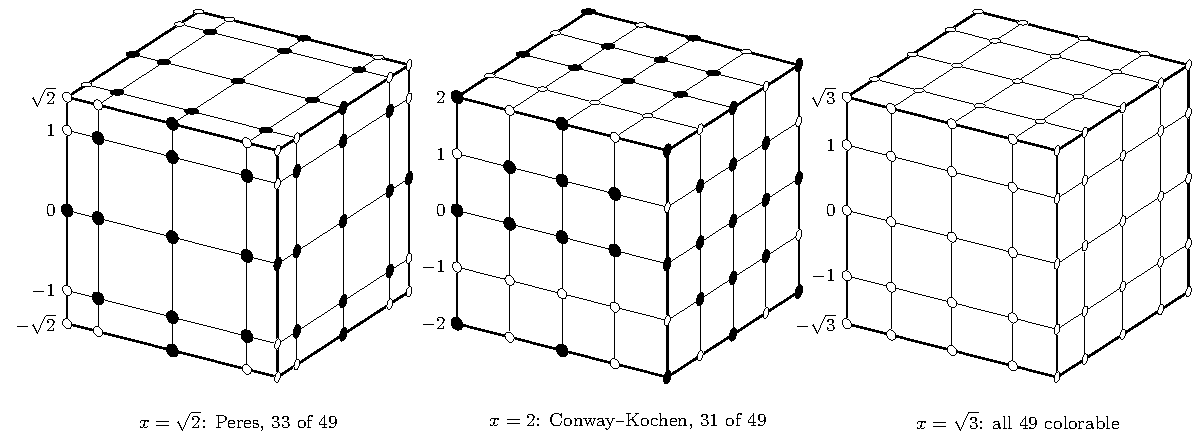
\includegraphics[width=\textwidth]{figures/alphabet_cube_triptych.pdf}
\caption{One cube, three alphabets $\{0,\pm1,\pm x\}$ with $x$ real and $x>1$.  Each of the 49
rays of the pool leaves the centre through a grid point; antipodal points are the same ray.
Filled points: the 33 rays of Peres ($x=\sqrt2$, the unique smallest uncolorable subset of that
pool) and the 31 rays of Conway and Kochen ($x=2$, one of six smallest subsets, all equivalent
under signed permutations of the axes).  At $x=\sqrt3$ the whole pool is colorable.  Only the two
inner grid lines move with~$x$.  Nearness of two points on the cube says nothing about
orthogonality of the rays, and the picture does not represent the complex pools of
Section~\ref{sec:circle}.}
\label{fig:triptych}
\end{figure}

\begin{figure}[t]
\centering
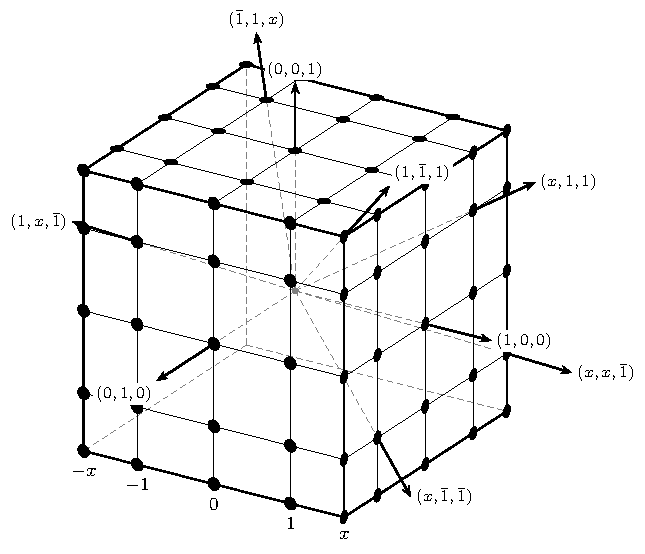
\includegraphics[width=0.6\textwidth]{figures/alphabet_cube_generic.pdf}
\caption{Words as rays.  A ray whose coordinates form a word over $\{0,\pm1,\pm x\}$ leaves the
centre of the cube $[-x,x]^3$ through a grid point; a bar is a minus sign.  Words without the
letter~$x$, such as $(1,0,0)$ and $(1,\bar1,1)$, reach the surface after scaling by~$x$.  The
49 rays are the same list of words for every~$x$; which pairs are orthogonal is not.  For
example $(x,1,1)\cdot(x,\bar1,\bar1)=x^2-1-1$, which vanishes only for $x^2=2$.}
\label{fig:generic}
\end{figure}

\paragraph{What this version claims.}
Versions 1--9 of this paper proposed that KS-uncolorability of a pool is governed by a small
number of ``cancellation mechanisms'' with a bound on the size of the generator, and that the
uncolorable alphabets form isolated ``islands''.  A full re-examination, by the author with two
language models acting as adversarial referees, found that proposal untenable: its central
statement is true by definition, its bound is contradicted by the paper's own examples, its
isolation claim is false, and one of its certified minima was wrong
(Section~\ref{sec:corrections} gives the full list).  The algorithm used to certify minima was
unsound.  Version~10 keeps the alphabet as the object of study and replaces the rest:

\begin{enumerate}[label=(\roman*)]
\item Three theorems.  Theorem~\ref{thm:twosymbol}: for every complex $x$ the pool of the
two-symbol alphabet $\{0,\pm1,\pm x\}$ is classified, and none contains a KS set of fewer than
31 rays.  Theorem~\ref{thm:6n}: the roots-of-unity pool is uncolorable exactly when
$6\mid n$.  Theorem~\ref{thm:circle}: the conjugate-closed pool over $\{0,\pm1,\pm x,\pm x^{*}\}$
is uncolorable for every $x$ on the circle $|x|^2=2$ and colorable for generic~$x$, with an
explicit smallest list of 45 words that works along the whole circle.
\item A catalogue of named finite pools (Section~\ref{sec:catalogue}), each with exact counts and
either a certified minimum KS subset or a stated upper bound, all recomputed for this version
with a certification procedure whose soundness argument is given in Section~\ref{sec:methods}.
\item A complete enumeration of the short vanishing sums available to a two-symbol alphabet
(Table~\ref{tab:zerosums}), replacing a list that had been compiled by inspection.
\end{enumerate}

Earlier versions called an uncolorable alphabet an ``island''.  Since the alphabets in question
turn out not to be isolated, this version does not use the word.

\section{Definitions and methods}\label{sec:prelim}

\begin{definition}
A \emph{ray} in $\C^3$ is a one-dimensional subspace, written $[v]$ for a nonzero vector~$v$.
Rays $[v],[w]$ are \emph{orthogonal} if $\braket vw=\sum_k v_k^{*}w_k=0$.  A \emph{triad} (or
\emph{basis}) is a set of three mutually orthogonal rays.
\end{definition}

\begin{definition}
A \emph{coloring} of a set $S$ of rays is a map $f:S\to\{0,1\}$ such that (a)~no two orthogonal
rays of $S$ both receive~1, and (b)~every triad contained in $S$ has exactly one ray with value~1.
$S$ is \emph{KS-uncolorable}, or a \emph{KS set}, if it has no coloring.  Its \emph{orthogonality
graph} has the rays as vertices and the orthogonal pairs as edges; the triads are its triangles.
Both the edges and the triangles enter the definition, and an edge lying in no triangle of $S$
is still a constraint.
\end{definition}

A coloring of $S$ restricts to a coloring of any subset, because every orthogonal pair and every
triad of the subset is one of~$S$:

\begin{lemma}[Restriction]\label{lem:restrict}
A set of rays that contains an uncolorable subset is uncolorable.
\end{lemma}

\begin{definition}
An \emph{alphabet} is a finite set $\mathcal A\subset\C$ containing~0.  Its \emph{raw pool} is
\[
S(\mathcal A)=\{\,[v]: v\in\mathcal A^3\setminus\{0\}\,\}.
\]
The \emph{completed pool} $\bar S(\mathcal A)$ is the smallest set of rays containing
$S(\mathcal A)$ and containing, with every orthogonal pair $[v],[w]$, the third ray of their
triad, $[(v\times w)^{*}]$ (the ordinary cross product for real vectors).  In all cases reported
here the completion was computed to closure and is finite; we do not know a general finiteness
criterion.
\end{definition}

In a completed pool every orthogonal pair lies in exactly one triad, so the numbers of pairs $E$
and triads $T$ satisfy $E=3T$.  This is a convenient check: the raw Eisenstein pool has
$E=174$, $T=22$, so it is not closed, contrary to a statement in version~9.

\paragraph{Three cautions on scope.}
(1)~Uncolorability is a property of a pool, not of a ring or a field.  Every ring that appears in
this paper contains $\Z$ and therefore contains the coordinates of $\CK$; the statement ``this
field supports a KS set'' is true of all of them and distinguishes nothing.  (2)~The size of a
generator is not an invariant of the pool: multiplying every word by $x^{-1}$ shows
$S(\{0,\pm1,\pm x\})=S(\{0,\pm1,\pm x^{-1}\})$, and $S$ is also unchanged by $x\mapsto-x$.
(3)~A raw pool and its completion are different objects; a statement about one says nothing about
the other, and every count below says which is meant.

\subsection{Methods}\label{sec:methods}

\paragraph{Exact arithmetic.}  Coordinates are elements of a number field $\Q[t]/(m(t))$ stored
as rational coefficient vectors; rays are compared after division by the first nonzero
coordinate; a pair is orthogonal when the Hermitian product is the zero element.  The
cyclotomic pools use exponents modulo~$n$, and the proof of Theorem~\ref{thm:circle} uses
integer polynomial identities.  No count in Sections~\ref{sec:real}--\ref{sec:catalogue} depends
on a floating-point tolerance.  The only floating-point quantities in the paper are the rigidity ranks of
Table~\ref{tab:rigidity}, including the coordinates of the 45-word set used there; they are
labelled as numerical.

\paragraph{Colorability.}  Colorability of a finite set is decided by a SAT
solver~\cite{AudemardSimon2018}: one variable per ray, a clause forbidding two 1s on each
orthogonal pair, and a clause requiring at least one 1 on each triad.

\paragraph{Certified minima.}  Let $P$ be an uncolorable pool.  If $M\subseteq P$ is colorable
then, by Lemma~\ref{lem:restrict}, every uncolorable subset of $P$ contains a ray outside~$M$.
The certifier keeps a list of such sets $M$, each verified colorable by the SAT solver, and asks
a second solver for a set $R$ of fewer than $u$ rays meeting the complement of every listed~$M$,
where $u$ is the size of the best uncolorable subset found so far.  If $R$ is uncolorable, $u$
decreases; if $R$ is colorable it is enlarged to a colorable set $M\supseteq R$ and $M$ joins the
list.  When no such $R$ exists, no uncolorable subset has fewer than $u$ rays, and the minimum is
exactly~$u$.  The answer is correct whenever the SAT solver is.  The list of sets $M$ is in principle a
certificate that can be checked independently; in this version it is archived only for
Theorem~\ref{thm:circle}, and the other minima are reproducible by re-running the scripts.  Minima that the procedure did not finish within
its time budget are reported as upper bounds.  The same enumeration, continued after the first
minimum set is found, lists \emph{all} minimum sets of a pool.

The procedure used in earlier versions (described there as ``OCUS'') was different and was not
sound: when a candidate was colorable, it required the next candidate to contain a ray that
completes a violated triad with \emph{two} rays of the current candidate, ignoring triads with
two or three rays outside it.  That can exclude genuine uncolorable subsets, and it did: it
reported 52 for the completed golden-ratio pool, which contains an uncolorable subset of~51.
None of the minima in this version comes from that code.

\section{Two-symbol alphabets}\label{sec:real}

The alphabets of Peres and of Conway and Kochen are both of the form $\{0,\pm1,\pm x\}$.  For any
$x\notin\{0,\pm1\}$ this alphabet has $5^3-1=124$ words, the same list for every~$x$
(Fig.~\ref{fig:generic}).  They give 49 rays for every $x$ other than $\pm i$, where more
words coincide and 31 remain (Theorem~\ref{thm:twosymbol}).  What depends on $x$ is which
inner products vanish.

\subsection{Which inner products can vanish}

A term of the inner product of two words is $a^{*}b$ with $a,b$ letters, so it is zero or one of
$\pm1,\ \pm x,\ \pm x^{*},\ \pm|x|^2$.  An inner product is therefore
\[
c_0+c_1x+c_2x^{*}+c_3|x|^2,\qquad c_i\in\Z,\quad |c_0|+|c_1|+|c_2|+|c_3|\le 3 .
\]
Some of these vanish for every $x$ (all $c_i=0$: disjoint supports, or terms cancelling in
pairs).  The others vanish only for special~$x$, and since there are finitely many coefficient
vectors they can be listed completely.  There are 128 nonzero vectors.  The pool is unchanged by
$x\mapsto-x$ and by $x\mapsto1/x$, and complex conjugation of all coordinates carries it to the
pool of $x^{*}$, which has the same orthogonality graph.  Together with an overall sign these
maps act on the coefficient vectors, inversion as
$(c_0,c_1,c_2,c_3)\mapsto(c_3,c_2,c_1,c_0)$.  The 128 vectors fall into 21 orbits, of which 13
have no solution other than $x\in\{0,\pm1\}$.  Table~\ref{tab:zerosums} lists the remaining
eight.

\begin{table}[t]
\centering
\caption{Every relation of at most three terms that can make an inner product of two words over
$\{0,\pm1,\pm x\}$ vanish for some but not all $x$, up to the symmetries $x\mapsto-x$,
$x\mapsto x^{*}$, $x\mapsto1/x$ and overall sign (computed by \texttt{ks\_zero\_sums\_v10.py}).
The row $x-x^{*}=0$ is the reason real alphabets have orthogonalities that generic complex ones
lack.
The rows $2+x=0$ and $1+2x=0$ describe the same pool, since $S$ is unchanged by $x\mapsto 1/x$.
A row says where extra orthogonalities appear; it says nothing by itself about colorability.}
\label{tab:zerosums}
\begin{tabular}{@{}rlll@{}}
\toprule
Terms & Representative relation & Orbit size & Solution set \\
\midrule
2 & $1-|x|^2=0$ & 2 & $|x|^2=1$ \\
2 & $x+x^{*}=0$ & 2 & $\mathrm{Re}\,x=0$ \\
2 & $x-x^{*}=0$ & 2 & $\mathrm{Im}\,x=0$ \\
3 & $2+x=0$ & 16 & $x=-2$ \\
3 & $2-|x|^2=0$ & 4 & $|x|^2=2$ \\
3 & $1+2x=0$ & 16 & $x=-1/2$ \\
3 & $1+x+x^{*}=0$ & 8 & $\mathrm{Re}\,x=-1/2$ \\
3 & $1+x-|x|^2=0$ & 8 & $x=(1\pm\sqrt{5})/2$ \\
\bottomrule
\end{tabular}

\end{table}

Three remarks.  First, the solution sets are not isolated points in general: two of them are
circles and three are lines in the complex plane.  Second, the two-term relations were missing
from the corresponding table of earlier versions; the relation $x+x^{*}=0$ was pointed out to us
by Frembs~\cite{Frembs2026}.  It holds on the imaginary axis, as $x-x^{*}=0$ holds on the real
axis, and the two classical modulus-2 alphabets differ in exactly this.  Of the 120 orthogonal
pairs of the $\sqrt{-2}$ pool (in the word representatives used here), 60 hold for every $x$, 54
use $x+x^{*}=0$ and 6 use $|x|^2=2$; at $x=\sqrt2$ the 54 are replaced by pairs using
$x-x^{*}=0$.  The difference is visible in the graphs (Computed fact~\ref{fact:pools}).  Third, the statement that an
uncolorable pool must have some vanishing inner products of this kind is true by definition and
has no content; versions 1--9 presented it as a finding.  The content is in which loci give
uncolorable pools, and that has to be computed.

\subsection{Real alphabets}

\begin{table}[t]
\centering
\caption{Raw pools of two-symbol alphabets $\{0,\pm1,\pm x\}$, exact arithmetic.  ``Min'' is the
certified size of the smallest uncolorable subset.  Every real $x=\sqrt d$ with $d$ a non-square
integer, $3\le d\le30$, gives the same counts as $\sqrt3$, as do $x=3$, $x=4$ and
$x=(1+\sqrt d)/2$ for $d=13,17,21,29$.}
\label{tab:alphabets}
\begin{tabular}{lrrrcc}
\toprule
Alphabet & Rays & Pairs & Triads & Colorable & Min \\
\midrule
$\{0,\pm1\}$ & 13 & 24 & 4 & yes & --- \\
$\{0,\pm1,\pm2\}$ (also $\pm\tfrac12$) & 49 & 138 & 26 & \textbf{no} & \textbf{31} \\
$\{0,\pm1,\pm\sqrt2\}$ & 49 & 120 & 16 & \textbf{no} & \textbf{33} \\
$\{0,\pm1,\pm\sqrt3\}$ & 49 & 114 & 10 & yes & --- \\
$\{0,\pm1,\pm\varphi\}$, $\varphi=(1+\sqrt5)/2$ & 49 & 138 & 10 & yes & --- \\
\midrule
$\{0,\pm1,\pm\sqrt{-1}\}$ & 31 & 69 & 7 & yes & --- \\
$\{0,\pm1,\pm\sqrt{-2}\}$ & 49 & 120 & 16 & \textbf{no} & \textbf{33} \\
$\{0,\pm1,\pm\sqrt{-d}\}$, $d=3,5,6,\dots,15$ & 49 & 114 & 10 & yes & --- \\
\bottomrule
\end{tabular}
\end{table}

Table~\ref{tab:alphabets} gives the raw pools.  The 13-ray pool of $\{0,\pm1\}$ is colorable, as
it must be: 13 is below the lower bound of~24.  Among real two-symbol alphabets the
only uncolorable raw pools are those of $x=2$ and $x=\sqrt2$ (and their negatives and
reciprocals), the two alphabets of Peres's cubes; Theorem~\ref{thm:twosymbol} below proves this
for every real~$x$ and settles the complex case as well.
The row for $\sqrt{-1}$ corrects version~9, which printed 25 rays; every nonzero letter of that
alphabet is a unit, the group $\{\pm1,\pm i\}$ acts freely on the 124 words, and $124/4=31$.

\begin{fact}[Integer pool]\label{fact:integer}
The 49-ray pool of $\{0,\pm1,\pm2\}$ has minimum uncolorable subsets of 31 rays, certified.  There
are exactly six such subsets.  They form a single orbit under the 48 signed permutations of the
coordinates, so all six are copies of $\CK$.  Together they use 37 of the 49 rays; the 12 unused
rays are those of squared length~9, such as $(1,2,2)$; 13 rays, those of $\{0,\pm1\}$, lie in all
six.  The completed pool has 109 rays, 258 pairs and 86 triads, and its minimum is also 31,
certified.
\end{fact}

Version~9 stated that the pool contains 162 distinct minimal sets falling into six classes.  The
exhaustive enumeration gives six sets in one class.  The pool also contains uncolorable subsets
that are critical (no ray can be removed) but not of minimum size, among them the 33-ray set
of Sch\"utte, also known as the Conway--Kochen 33-ray set and communicated by them to
Peres~\cite{Peres1991} (the identification is made in~\cite{TrandafirCabello2025}), which has 76
orthogonal pairs and
20 bases and is contained in the 37 rays above.

None of three enlargements we tried lowers the minimum: the raw pools of $\{0,\pm1,\pm2,\pm3\}$ (145 rays),
$\{0,\pm1,\pm\sqrt2,\pm2\}$ (109 rays) and $\{0,\pm1,\pm\varphi,\pm2\}$ (145 rays) all have
certified minimum 31, with 17 bases in the minimum set found, while
$\{0,\pm1,\pm\varphi,\pm\varphi^2\}$ (109 rays, 24 triads) is colorable.  Each of the first three
contains the integer pool, so 31 is an upper bound by Lemma~\ref{lem:restrict}; the content of
the computation is that nothing smaller appears.

\begin{fact}[Peres pool]\label{fact:peres}
The 49-ray pool of $\{0,\pm1,\pm\sqrt2\}$ has a unique minimum uncolorable subset, the 33 rays of
Peres (72 pairs, 16 bases).  The other 16 rays lie in no triad.  The completed pool has 145 rays,
336 pairs and 112 triads, and its minimum is 33, certified.  The same statements hold for
$\{0,\pm1,\pm\sqrt{-2}\}$.
\end{fact}

\begin{fact}[The two modulus-2 pools are not the same graph]\label{fact:pools}
The minimum 33-ray sets of the $\sqrt2$ and $\sqrt{-2}$ pools have isomorphic orthogonality
graphs.  The two 49-ray pools do not, although they agree in the number of rays, pairs, triads,
in degree sequence and in spectrum; neither do the two 145-ray completed pools.  (Graph
isomorphism was tested with VF2~\cite{Cordella2004VF2}; for the raw pools we also checked directly
that none of the 48 isomorphisms between the two 33-ray cores carries the neighbourhoods of the
other 16 rays of one pool onto those of the other.)
\end{fact}

Versions 1--9 called these two alphabets ``isomorphic islands''.  That is correct for the
minimum sets and false for the pools.  The difference is the one Frembs identified: 54 of the 120
orthogonalities of the $\sqrt{-2}$ pool use $x+x^{*}=0$, a relation that fails at $x=\sqrt2$, and
he builds an arrangement on that relation~\cite{Frembs2026}.

\subsection{All two-symbol alphabets}\label{sec:twosymbol}

The completeness of Table~\ref{tab:zerosums} turns the question ``for which $x$ is the pool of
$\{0,\pm1,\pm x\}$ uncolorable?'' into a finite computation, and the answer is a theorem about
every complex~$x$.

\begin{theorem}[Two-symbol alphabets]\label{thm:twosymbol}
Let $x$ be a nonzero complex number and $S(x)$ the pool of all words over $\{0,\pm1,\pm x\}$.
\begin{enumerate}[label=(\roman*)]
\item $S(x)$ is uncolorable if and only if $x$ or $1/x$ is one of $\pm2$, $\pm\sqrt2$,
$\pm\sqrt{-2}$, or $x$ is a primitive third or sixth root of unity.
\item The minimum uncolorable subset of $S(x)$ has 31 rays for $x\in\{\pm2,\pm\tfrac12\}$, where
the minimum sets are the six copies of $\CK$ of Computed fact~\ref{fact:integer}, and 33 rays in
every other uncolorable case.
\item Consequently, if all rays of a KS set have coordinates in $\{0,\pm a,\pm b\}$ for some
complex numbers $a$ and $b$, the set has at least 31 rays.
\end{enumerate}
\end{theorem}

\begin{proof}
Write $x=a+ib$.  The orthogonality graph of $S(x)$ depends on $x$ only through two finite pieces
of data: which words are proportional, and which inner products vanish.

\emph{Proportionality.}  Two words are proportional when their three $2\times2$ minors vanish.
A minor is a difference of two products of two letters, and such a product is $0$, $\pm1$, $\pm x$ or $\pm x^2$.  So a minor is identically zero, or a
monomial or twice a monomial (never zero), or one of $\pm(1\pm x)$, $\pm(1\pm x^2)$,
$\pm x(1\pm x)$.  Away from $x\in\{\pm1,\pm i\}$
the same words are proportional for every~$x$, and the pool has 49 rays.

\emph{Orthogonality.}  An inner product is $c_0+c_1x+c_2x^{*}+c_3|x|^2$ for one of the 128
coefficient vectors counted above, or is identically zero.  It vanishes when
$(c_1-c_2)\,b=0$ and $c_0+(c_1+c_2)\,a+c_3(a^2+b^2)=0$.  For a given vector the solution set is
therefore empty, a finite set of real points, the real axis, a vertical line, or a circle
centred on the real axis.  Going through the 128 vectors gives nine curves,
\[
\mathrm{Im}\,x=0,\quad \mathrm{Re}\,x=0,\ \pm\tfrac12,\quad |x|^2=\tfrac12,\ 1,\ 2,\quad
|x\pm1|=1,
\]
and finitely many real points.  Call a point \emph{special} if it is one of those real points, a
point of intersection of two of the curves, or one of $\pm1,\pm i$.  There are 27 special points
up to complex conjugation.  At a point that is not special and lies on none of the curves, no
vector vanishes.  At a point of a curve $C$ that is not special, the vectors that vanish are
exactly those whose solution set is~$C$, since any other vector vanishes on a different curve or
on special points only.  Hence the graph of $S(x)$ is constant on the complement of the curves,
constant on each curve away from the special points, and otherwise has to be computed at each
special point: $1+9+27=37$ cases.  (Conjugating all coordinates carries $S(x)$ to $S(x^{*})$ and
preserves orthogonality, so $x$ and $x^{*}$ need not be distinguished.)

\emph{Computation.}  The script \texttt{ks\_two\_symbol\_theorem.py} lists the curves and special
points, takes an exact sample point on each curve, builds the 37 graphs in exact arithmetic, decides colorability of each, and runs the certification procedure of
Section~\ref{sec:methods} on every uncolorable one; all terminate.
Table~\ref{tab:twosymbol} is the result, with the cases grouped by the symmetries $x\mapsto-x$
and $x\mapsto1/x$, which do not change the pool.  Parts (i) and (ii) are read off the table.  For
(iii), if $a$ or $b$ is zero or $a=\pm b$ the rays lie in the 13-ray pool of $\{0,\pm1\}$, which
is colorable; otherwise dividing all coordinates by $a$ puts the set inside $S(b/a)$.
\end{proof}

\begin{table}[t]
\centering
\caption{Every pool of a two-symbol alphabet $\{0,\pm1,\pm x\}$, $x\in\mathbb{C}\setminus\{0\}$
(Theorem~\ref{thm:twosymbol}).  A curve stands for its points other than the special points
listed below it.  ``Min'' is the certified size of the smallest uncolorable subset, and the last
column names the graph of the minimum set found (isomorphism by VF2).}
\label{tab:twosymbol}
\small
\begin{tabular}{@{}lrrrcl@{}}
\toprule
$x$ & Rays & Pairs & Triads & Min & Minimum set \\
\midrule
on no curve & 49 & 60 & 4 & --- & colorable \\
$\mathrm{Im}\,x=0$;\ \ $\mathrm{Re}\,x=0$;\ \ $|x|=1$ & 49 & 114 & 10 & --- & colorable \\
$\mathrm{Re}\,x=\pm\tfrac12$;\ \ $|x\pm1|=1$ & 49 & 72 & 8 & --- & colorable \\
$|x|^2=2$;\ \ $|x|^2=\tfrac12$ & 49 & 66 & 10 & --- & colorable \\
\midrule
$\pm1$ & 13 & 24 & 4 & --- & colorable \\
$\pm i$ & 31 & 69 & 7 & --- & colorable \\
$\pm\varphi,\ \pm1/\varphi$ & 49 & 138 & 10 & --- & colorable \\
$\pm1\pm i,\ (\pm1\pm i)/2$ & 49 & 78 & 14 & --- & colorable \\
$(\pm1\pm\sqrt{-7})/2,\ (\pm1\pm\sqrt{-7})/4$ & 49 & 78 & 14 & --- & colorable \\
$\pm2,\ \pm\tfrac12$ & 49 & 138 & 26 & \textbf{31} & $\CK$ \\
$\pm\sqrt2,\ \pm1/\sqrt2$ & 49 & 120 & 16 & \textbf{33} & Peres \\
$\pm\sqrt{-2},\ \pm1/\sqrt{-2}$ & 49 & 120 & 16 & \textbf{33} & Peres \\
$(\pm1\pm\sqrt{-3})/2$ & 49 & 138 & 18 & \textbf{33} & Eisenstein 33 \\
\bottomrule
\end{tabular}
\end{table}

Four remarks on what the theorem does and does not say.

First, it is a statement about a class of coordinate systems, not about KS sets in general.
The minimum number of rays of a KS set in dimension three is known only to lie between 24
and~31, and a set smaller than 31, if one exists, would need at least three nonzero letters up to
sign.  What the theorem
shows is that the construction read off Peres's cubes, one unit and one further number along
each axis, cannot beat Conway and Kochen whatever the number is.

Second, it concerns the raw pool.  Completion adds rays whose coordinates are not letters, and
the completed pool of $\{0,\pm1,\pm\varphi\}$ is uncolorable although its raw pool is not
(Section~\ref{sec:catalogue}).

Third, the uncolorable cases are isolated points; no curve of Table~\ref{tab:zerosums} is
uncolorable for a two-symbol alphabet.  In particular the two-symbol pool is colorable at a
generic point of the circle $|x|^2=2$, and even at $x=1+i$ and $x=(1+\sqrt{-7})/2$, where it
meets another curve.  The uncolorability of that whole circle (Theorem~\ref{thm:circle}) needs the
conjugate letter $x^{*}$.

Fourth, the last row did not appear in earlier versions.  At a primitive sixth root of unity three curves
meet ($|x|=1$, $\mathrm{Re}\,x=\tfrac12$, $|x-1|=1$), and the 49 rays over $\{0,\pm1,\pm\omega\}$
are already uncolorable, with a minimum set isomorphic to the Eisenstein 33-ray set of
Section~\ref{sec:roots}.  The letter $\omega^2$ of the Eisenstein alphabet is not needed.

\section{Roots of unity}\label{sec:roots}

Let $\zeta_n=e^{2\pi i/n}$, let $\mu_n$ be the group of $n$th roots of unity, and put
$S_n=S(\{0\}\cup\mu_n)$.  The case $n=6$ is the alphabet $\{0,\pm1,\pm\omega,\pm\omega^2\}$ with
$\omega=e^{2\pi i/3}$, which contains the 33-ray set that Cabello calls the simplest KS
set~\cite{Cabello2025simplest}.

\begin{lemma}\label{lem:sums}
A sum of two elements of $\mu_n$ can vanish if and only if $2\mid n$.  A sum of three can vanish
if and only if $3\mid n$, and then the three terms are $\beta,\beta\omega,\beta\omega^2$ for some
$\beta\in\mu_n$.
\end{lemma}

\begin{proof}
$\zeta^a+\zeta^b=0$ iff $\zeta^{b-a}=-1$, and $-1\in\mu_n$ iff $2\mid n$.  For three terms divide
by the first: $1+e^{i\theta}+e^{i\phi}=0$.  The imaginary part gives $\phi=-\theta$ or
$\phi=\pi+\theta$; the second makes the real part equal to~1.  With $\phi=-\theta$ the real part
gives $\cos\theta=-\tfrac12$, so the other two terms are $\omega$ and $\omega^2$, which lie in
$\mu_n$ iff $3\mid n$.
\end{proof}

Hence two rays of $S_n$ are orthogonal only if the number of coordinates in which both are
nonzero is~0, or~2 with $2\mid n$, or~3 with $3\mid n$.

\begin{theorem}\label{thm:6n}
$S_n$ is KS-uncolorable if and only if $6\mid n$.
\end{theorem}

\begin{proof}
\emph{If.}  For $6\mid n$ we have $\mu_6\subseteq\mu_n$ and so $S_6\subseteq S_n$.  The pool
$S_6$ is uncolorable (Table~\ref{tab:cyc}; it contains the 33-ray set
of~\cite{Cabello2025simplest}).  Apply Lemma~\ref{lem:restrict}.

\emph{Only if.}  Let $6\nmid n$ and write $e_1,e_2,e_3$ for the axis rays.

\emph{Case 1: $2\nmid n$ and $3\nmid n$.}  Orthogonal rays have disjoint supports, so the only
triad is $\{e_1,e_2,e_3\}$.  Give $e_1$ the value~1 and every other ray~0.

\emph{Case 2: $2\mid n$, $3\nmid n$.}  Two rays with three common nonzero coordinates are never
orthogonal.  No triad contains an all-nonzero ray~$a$: each of its two partners would share
exactly two nonzero coordinates with~$a$ and so have support of size~2; two such supports meet,
so the partners, being orthogonal to each other, would have the same support; and then $a$ would
be orthogonal to a basis of that coordinate plane and vanish on it.  Rays whose supports are
different two-element sets share one coordinate and are not orthogonal.  So every triad is
$\{e_1,e_2,e_3\}$ or $\{e_k,v,v'\}$ with $v,v'$ in the coordinate plane orthogonal to~$e_k$.  In
such a plane the rays are $(1,\zeta^p)$, and $(1,\zeta^p)\perp(1,\zeta^q)$ iff $q-p\equiv n/2$: a
perfect matching.  Give $e_1$ the value~1 and $e_2,e_3$ the value~0; give~0 to every ray of the
plane orthogonal to $e_1$; in each of the other two coordinate planes give~1 to one ray of each
matched pair and~0 to the other; give~0 to every all-nonzero ray.  Rays in different coordinate
planes are not orthogonal, and no ray with value~1 in those two planes is orthogonal to~$e_1$, so
no two rays with value~1 are orthogonal, and each triad has exactly one~1.

\emph{Case 3: $3\mid n$, $2\nmid n$.}  Orthogonality needs common support of size 0 or~3.  A ray
with exactly one zero coordinate is therefore orthogonal only to the axis ray on that coordinate,
and lies in no triad.  For an all-nonzero ray normalise $v=(1,a,b)$.  By Lemma~\ref{lem:sums} an
all-nonzero $w$ is orthogonal to $v$ iff $w=w_{\pm}=(1,a\omega^{\pm1},b\omega^{\mp1})$, and
$\braket{w_+}{w_-}=1+\omega^{-2}+\omega^{2}=0$.  So the all-nonzero rays fall into disjoint
triads, with no other orthogonalities among them and none to a ray with a zero coordinate.  Give
the value~1 to one ray of each such triad and to $e_1$, and~0 to everything else.
\end{proof}

The two primes do different work.  Divisibility by~3 creates triads: at $n=9$ and $n=15$ the pool
has 28 and 76 of them and is colorable because they are pairwise disjoint.  Divisibility by~2
creates the two-term cancellations that couple triads.  Only together do the constraints
interlock.  The fields $\Q(\zeta_3)$ and $\Q(\zeta_6)$ coincide, while $S_3$ is colorable and
$S_6$ is not: Theorem~\ref{thm:6n} is a statement about alphabets, not about fields, and it has
no formulation in terms of the Galois group of the field (the one offered in version~9 was
false).

\begin{table}[t]
\centering
\caption{Cyclotomic pools, exact arithmetic (exponents modulo $n$), colorability by SAT.  The
check was run for all $2\le n\le30$ and agrees with Theorem~\ref{thm:6n} in every case, as do the
three structural statements used in Cases 1--3; a selection is shown.}
\label{tab:cyc}
\begin{tabular}{rrrrc@{\qquad\qquad}rrrrc}
\toprule
$n$ & Rays & Pairs & Triads & Colorable & $n$ & Rays & Pairs & Triads & Colorable\\
\midrule
3 & 21 & 21 & 4 & yes & 12 & 183 & 633 & 67 & \textbf{no}\\
4 & 31 & 69 & 7 & yes & 15 & 273 & 273 & 76 & yes\\
5 & 43 & 18 & 1 & yes & 16 & 307 & 843 & 25 & yes\\
6 & 57 & 174 & 22 & \textbf{no} & 18 & 381 & 1380 & 136 & \textbf{no}\\
9 & 111 & 111 & 28 & yes & 20 & 463 & 1293 & 31 & yes\\
\bottomrule
\end{tabular}
\end{table}

\begin{fact}[Eisenstein pool]\label{fact:eisenstein}
The 57-ray pool $S_6$ has 174 orthogonal pairs and 22 triads.  Its minimum uncolorable subsets
have 33 rays, certified, and there are exactly three of them, each with 78 pairs and 14 bases.
The pool is not closed under completion: $(1,1,0)$ and $(1,\bar1,1)$ are orthogonal and their
third ray $(1,\bar1,\bar2)$ is not in $S_6$.  The completed pool has 165 rays, 390 pairs and 130
triads, and its minimum is also 33, certified.
\end{fact}

Since every $S_n$ with $6\mid n$ contains $S_6$, its minimum is at most~33.  We have not
certified the minimum for $n>6$.

\begin{remark}
Cortez, Morales and Reyes~\cite{CortezMoralesReyes2022} showed that $\Z[1/6]$ is the smallest
ring $\Z[1/N]$ over which the partial ring of symmetric $3\times3$ matrices admits no algebraic
hidden state.  The number~6 appears there
and in Theorem~\ref{thm:6n}, but the two statements concern different objects (matrix entries of
projectors in one, coordinates of rays in the other) and we know of no map from one to the
other.  Version~9 presented this as a quantitative connection; it is a coincidence until someone
proves otherwise.
\end{remark}

\section{The circle $|x|^2=2$}\label{sec:circle}

The two uncolorable alphabets $\{0,\pm1,\pm\sqrt2\}$ and $\{0,\pm1,\pm\sqrt{-2}\}$ both have
$|x|^2=2$, and in both the conjugate $x^{*}=\pm x$ is already a letter.  For a general complex
$x$ the alphabet that is closed under conjugation is
\[
\mathcal A(x)=\{0,\pm1,\pm x,\pm x^{*}\},\qquad P(x)=S(\mathcal A(x)).
\]
For generic $x$ the pool $P(x)$ has 145 rays; at special $x$ some of them coincide (49 remain
at $x=\sqrt{\pm2}$).  Versions 1--9 used this alphabet at one
point, $x=(1+\sqrt{-7})/2$, found the pool uncolorable, and attributed that to the arithmetic of
the ring of integers of $\Q(\sqrt{-7})$.  It is a property of the whole circle.  This section
proves that (Theorem~\ref{thm:circle}) and then determines every $x$ at which $P(x)$ is
uncolorable (Theorem~\ref{thm:conj}).

\begin{theorem}\label{thm:circle}
Let $W$ be the list of 45 words in Table~\ref{tab:words}.
\begin{enumerate}
\item[(i)] For every $x\in\C$ with $|x|^2=2$ the rays of $W$ form a KS-uncolorable set.
Consequently $P(x)$ is uncolorable for every such~$x$.
\item[(ii)] The orthogonalities among the 145 words that hold for every $x\in\C$ form a colorable
configuration (366 pairs, 22 triads).  Hence $P(x)$ is colorable for every $x$ outside a finite
union of proper real algebraic subsets of~$\C$.
\item[(iii)] No list of fewer than 45 of the 145 words is uncolorable by virtue of the
orthogonalities that hold along the whole circle.  Consequently no fixed list of fewer than 45
words over $\mathcal A(x)$ is uncolorable at every point of the circle.
\end{enumerate}
Part~(iii) concerns fixed lists of words over this alphabet.  It says nothing about other
parametrized families of KS sets.
\end{theorem}

\begin{proof}
The inner product of two words is a polynomial in $x$ and $x^{*}$ with integer coefficients, of
degree at most~2.

(i)  On the circle, $xx^{*}=2$ reduces every such polynomial to an integer combination of
$1,x,x^{*},x^2,x^{*2}$.  With $x=\sqrt2e^{i\theta}$ these are constant multiples of
$e^{ik\theta}$, $k=0,\pm1,\pm2$, which are linearly independent functions of~$\theta$.  So an
inner product vanishes at every point of the circle if and only if every reduced coefficient is
zero, a finite check in integers.  It yields 98 pairs among the words of $W$ that are orthogonal
at every point of the circle, forming the 22 triads listed in Appendix~\ref{app:triads}.  A SAT
solver shows that the configuration with these 98 exclusions and 22 triads has no coloring.  Now
fix $x$ on the circle.  If the 45 words give 45 distinct rays, the orthogonality graph at $x$
contains the 98 pairs, and any further pairs or triads only add constraints, so there is no
coloring.  If two words give the same ray, a coloring at $x$ assigns them the same value and so
would also be a coloring of the 45-vertex configuration; there is none.  (Two words that are
orthogonal for every $x$ on the circle cannot coincide at any point of it.)

(ii)  Without the relation, the monomials $x^ax^{*b}$ are linearly independent functions
on~$\C$, so an inner product vanishes for all $x$ iff all its coefficients vanish.  This yields
366 pairs and 22 triads on the 145 words, and a SAT solver finds a coloring.  Each remaining
inner product is a nonzero polynomial in $x,x^{*}$ and vanishes only on a proper real algebraic
subset.  For each pair of the 145 words at least one $2\times2$ minor of the pair is a nonzero
polynomial, so the set of $x$ at which the two words give the same ray is also a proper real
algebraic subset.  Away from those finitely many subsets the 145 rays are distinct, no further
pair is orthogonal, and the coloring found is a coloring of $P(x)$.

(iii)  The 145 words with the pairs and triads that hold along the whole circle (378 pairs, 34
triads) form a finite configuration, and the certifier of Section~\ref{sec:methods} returns 45 as
its minimum, with a certificate of 408 colorable sets.  For the consequence: the exceptional
points of the circle, at which some further inner product vanishes or two words coincide, are
finite in number, since each such condition is a nonzero trigonometric polynomial in~$\theta$.
A list uncolorable at every point of the circle is uncolorable at a non-exceptional point, where
the configuration is exactly the one just described.

The script \texttt{ks\_modulus2\_circle.py} carries out all three computations.  Its
output file, \texttt{results/modulus2\_circle.json}, holds the 145 words, both graphs, the
coloring of part~(ii) and the certificate of part~(iii).
\end{proof}

\begin{table}[t]
\centering
\caption{The 45 words of Theorem~\ref{thm:circle}.  A bar is a minus sign and $x^{*}$ is the
complex conjugate, so $\bar x^{*}=-x^{*}$.  The list is one minimum set; we have not enumerated
the others.}
\label{tab:words}
\small
\begin{tabular}{rl@{\qquad}rl@{\qquad}rl@{\qquad}rl@{\qquad}rl}
\hline
1 & $0\,0\,1$ & 10 & $1\,0\,1$ & 19 & $1\,1\,x^{*}$ & 28 & $1\,x^{*}\,\bar 1$ & 37 & $x\,\bar 1\,0$ \\
2 & $0\,1\,0$ & 11 & $1\,0\,\bar 1$ & 20 & $1\,1\,\bar x^{*}$ & 29 & $1\,\bar x^{*}\,0$ & 38 & $x\,\bar 1\,1$ \\
3 & $0\,1\,1$ & 12 & $1\,0\,x$ & 21 & $1\,\bar 1\,0$ & 30 & $1\,\bar x^{*}\,1$ & 39 & $x\,\bar 1\,\bar 1$ \\
4 & $0\,1\,\bar 1$ & 13 & $1\,0\,\bar x$ & 22 & $1\,\bar 1\,x$ & 31 & $1\,\bar x^{*}\,\bar 1$ & 40 & $x^{*}\,0\,1$ \\
5 & $0\,1\,x$ & 14 & $1\,0\,x^{*}$ & 23 & $1\,\bar 1\,\bar x$ & 32 & $x\,0\,1$ & 41 & $x^{*}\,0\,\bar 1$ \\
6 & $0\,1\,\bar x$ & 15 & $1\,0\,\bar x^{*}$ & 24 & $1\,\bar 1\,x^{*}$ & 33 & $x\,0\,\bar 1$ & 42 & $x^{*}\,1\,1$ \\
7 & $0\,x^{*}\,1$ & 16 & $1\,1\,0$ & 25 & $1\,\bar 1\,\bar x^{*}$ & 34 & $x\,1\,0$ & 43 & $x^{*}\,1\,\bar 1$ \\
8 & $0\,x^{*}\,\bar 1$ & 17 & $1\,1\,x$ & 26 & $1\,x^{*}\,0$ & 35 & $x\,1\,1$ & 44 & $x^{*}\,\bar 1\,1$ \\
9 & $1\,0\,0$ & 18 & $1\,1\,\bar x$ & 27 & $1\,x^{*}\,1$ & 36 & $x\,1\,\bar 1$ & 45 & $x^{*}\,\bar 1\,\bar 1$ \\
\hline
\end{tabular}

\end{table}

Comparing (i) and (ii): of the 378 pairs present along the circle, 366 are present for every
$x$, and the other 12 are all of the form $1+1-x^{*}x=0$, as in
$(x,1,1)\perp(x,\bar1,\bar1)$.  With them come 12 further triads.  These 12 pairs are the
difference between a colorable pool and an uncolorable one, and the relation behind them is the
one Peres's cube uses at $x=\sqrt2$ (Fig.~\ref{fig:generic}).

\begin{corollary}\label{cor:points}
\begin{enumerate}
\item[(a)] At $x=\sqrt2$ and at $x=\sqrt{-2}$ the 45 words give exactly 33 distinct rays.  By
Computed fact~\ref{fact:peres} these are the unique minimum sets of those pools; at $x=\sqrt2$
they are the 33 rays of Peres.
\item[(b)] At $x=(1+\sqrt{-7})/2$, $P(x)$ is the 145-ray pool studied in earlier versions.  It is
uncolorable because $|x|^2=2$.
\item[(c)] The words $(1,1,x)$ and $(1,0,x^{*})$ of $W$ have squared overlap
$|1+x^{*2}|^2/12=(5+4\cos2\theta)/12$, which is not constant.  The sets of part~(i) are therefore
not all unitarily equivalent: the multiset of squared overlaps between rays is a unitary
invariant that does not depend on labelling, and it takes infinitely many values along the
circle.
\item[(d)] At $x=(1+\sqrt{-7})/2$ the 45 words give 45 distinct rays with 114 orthogonal pairs
and 26 triads, and this set contains a 43-ray KS subset; 43 is the certified minimum within it.
\end{enumerate}
\end{corollary}

\begin{figure}[t]
\centering
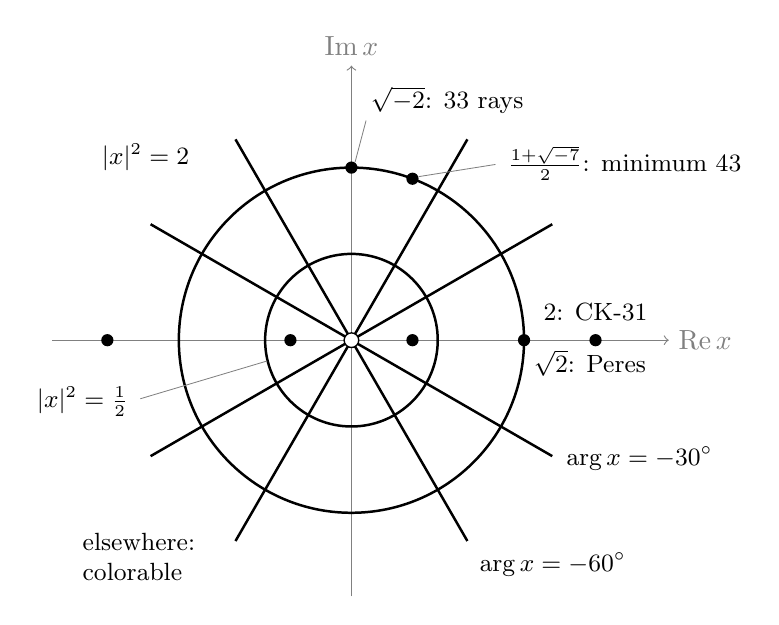
\begin{tikzpicture}[scale=1.55]
\draw[->,gray] (-2.45,0) -- (2.6,0) node[right] {$\mathrm{Re}\,x$};
\draw[->,gray] (0,-2.1) -- (0,2.25) node[above] {$\mathrm{Im}\,x$};
\foreach \t in {30,60,120,150} \draw[line width=0.9pt] (\t:-1.9) -- (\t:1.9);
\draw[line width=0.9pt] (0,0) circle (1.4142);
\draw[line width=0.9pt] (0,0) circle (0.7071);
\foreach \p in {-2,-0.5,0.5,2} \fill (\p,0) circle (0.05);
\draw[fill=white,line width=0.5pt] (0,0) circle (0.06);
\node[font=\small,anchor=south] at (2,0.08) {$2$: $\CK$};
\fill (1.4142,0) circle (0.05) node[below right,font=\small] {$\sqrt2$: Peres};
\fill (0,1.4142) circle (0.05);
\node[font=\small,anchor=south west] at (0.08,1.78) {$\sqrt{-2}$: 33 rays};
\draw[gray,line width=0.3pt] (0.03,1.46) -- (0.12,1.8);
\fill (0.5,1.3229) circle (0.05);
\node[font=\small,anchor=west] at (1.2,1.45) {$\tfrac{1+\sqrt{-7}}{2}$: minimum 43};
\draw[gray,line width=0.3pt] (0.55,1.34) -- (1.18,1.44);
\node[font=\small,anchor=east] at (-1.25,1.5) {$|x|^2=2$};
\node[font=\small,anchor=east] at (-1.75,-0.5) {$|x|^2=\tfrac12$};
\draw[gray,line width=0.3pt] (-0.69,-0.17) -- (-1.73,-0.48);
\node[font=\small,anchor=west] at (1.68,-0.97) {$\arg x=-30^\circ$};
\node[font=\small,anchor=north west] at (0.97,-1.66) {$\arg x=-60^\circ$};
\node[font=\small,align=left,anchor=north east] at (-1.2,-1.5) {elsewhere:\\colorable};
\end{tikzpicture}
\caption{The alphabet $\{0,\pm1,\pm x,\pm x^{*}\}$.  Its pool is uncolorable exactly on the set
drawn in black: the circles $|x|^2=2$ and $|x|^2=\tfrac12$, the four lines through the origin at
$\pm30^\circ$ and $\pm60^\circ$ to the real axis with the origin removed, and the points
$\pm2,\pm\tfrac12$ (Theorem~\ref{thm:conj}).  The pool is unchanged by $x\mapsto-x$ and
$x\mapsto x^{*}$, so one quadrant suffices.  At the four axis points of the outer circle, which
are two alphabets up to sign, the 45 words of Table~\ref{tab:words} collapse to 33 rays.  At $(1+\sqrt{-7})/2$ the additional
relation $x+x^{*}=1$ adds orthogonalities and the minimum drops from 45 to~43.}
\label{fig:circle}
\end{figure}

\subsection{The point $x=(1+\sqrt{-7})/2$}

Let $\alpha=(1+\sqrt{-7})/2$, so $|\alpha|^2=2$ and $\alpha+\alpha^{*}=1$.

\begin{fact}[The $\Q(\sqrt{-7})$ pool]\label{fact:heegner}
$P(\alpha)$ has 145 rays, 522 orthogonal pairs and 42 triads, against 378 and 34 at a generic
point of the circle.  Its minimum uncolorable subsets have 43 rays, certified.  There are exactly
six of them, in two orbits under signed permutations of the coordinates, each with 23 bases; the
one we use has 107 pairs and degree sequence $4^{16}5^{20}6^{4}8^{2}10^{1}$.  The completed pool
has 685 rays, 1746 pairs and 582 triads; its minimum is \heegnercompletedmin.
\end{fact}

So the additional relation at this point is worth two rays: 43 against 45
(Corollary~\ref{cor:points}d).  It is the pools $P(x)$ that form a continuous family through
this point.  Theorem~\ref{thm:circle} proves that $P(\alpha)$ is uncolorable; that its minimum is
43 is a separate computation.

Table~\ref{tab:heegner} puts this point in the setting in which earlier versions found it.  For
each of the nine imaginary quadratic fields of class number one we take the generator $a$ of the
ring of integers and the alphabet $\{0,\pm1,\pm a,\pm a^{*}\}$.  The uncolorable rows are
$d=2$ (a point of the circle), $d=3$ (the roots-of-unity alphabet $S_6$ of
Theorem~\ref{thm:6n}) and $d=7$ (a point of the circle).  Class number plays no role that we can
see; Theorems~\ref{thm:6n} and~\ref{thm:circle} account for all three rows.

\begin{table}[t]
\centering
\caption{Raw pools of $\{0,\pm1,\pm a,\pm a^{*}\}$, $a$ the generator of the ring of integers of
$\Q(\sqrt{-d})$: $a=\sqrt{-d}$ for $d=1,2$ and $a=(1+\sqrt{-d})/2$ otherwise.  Minima are
certified.  For $d=1$ version~9 printed a different, larger alphabet in this row; see the text.}
\label{tab:heegner}
\begin{tabular}{rcrrrcc}
\toprule
$d$ & $|a|^2$ & Rays & Pairs & Triads & Colorable & Min \\
\midrule
1 & 1 & 31 & 69 & 7 & yes & --- \\
2 & 2 & 49 & 120 & 16 & \textbf{no} & \textbf{33} \\
3 & 1 & 57 & 174 & 22 & \textbf{no} & \textbf{33} \\
7 & 2 & 145 & 522 & 42 & \textbf{no} & \textbf{43} \\
11, 19, 43, 67, 163 & $3,5,11,17,41$ & 145 & 462 & 30 & yes & --- \\
\bottomrule
\end{tabular}
\end{table}

For $d=1$ the letters are $0,\pm1,\pm i$ and the pool is $S_4$, colorable by
Theorem~\ref{thm:6n}.  The larger Gaussian alphabet $\{0,\pm1,\pm i,\pm(1+i)\}$, which contains
the element $1+i$ of squared modulus~2, generates 127 rays, 465 pairs and 51 triads; that pool is
uncolorable with certified minimum~33 (16 bases in the set found).

\subsection{Relation to the family of Gould and Aravind}

Gould and Aravind~\cite{GouldAravind2010} exhibited a family of 33-ray sets with the
orthogonality graph of Peres's set, depending on three phases, containing the sets of Peres and
of Penrose; Flores Gordillo~\cite{FloresGordillo2026} reports that after removing diagonal
unitaries the family is a circle (we have not audited that proof).  That family is different from the one in
Theorem~\ref{thm:circle}.  Its members have 33 rays and a constant graph.  Ours has 45 rays at a
generic point and cannot contain a 33-ray KS set there: every orthogonality of $P(x)$ at a generic
point of the circle is also one of $P(\alpha)$, whose minimum is~43, so no subset of $P(x)$ with
fewer than 43 rays is uncolorable.  (Theorem~\ref{thm:conj} below gives 45.)  The two families meet at $x=\sqrt2$, where both give Peres's
set.  We have not found the family of Theorem~\ref{thm:circle} in the literature, but we have not
made a systematic search and make no claim of priority.

\subsection{Every conjugate-closed alphabet}\label{sec:conjclosed}

Theorem~\ref{thm:circle} settles one curve in the plane of~$x$.  The method of
Theorem~\ref{thm:twosymbol} settles the plane.

\begin{theorem}[Conjugate-closed alphabets]\label{thm:conj}
Let $x$ be a nonzero complex number and $P(x)$ the pool of all words over
$\{0,\pm1,\pm x,\pm x^{*}\}$.
\begin{enumerate}[label=(\roman*)]
\item $P(x)$ is uncolorable if and only if one of the following holds:
\begin{enumerate}[label=(\alph*)]
\item $|x|^2=2$;
\item $|x|^2=\tfrac12$;
\item $x^{*}/x$ is a primitive third or sixth root of unity, that is, $\arg x$ is one of
$\pm30^\circ$, $\pm60^\circ$, $\pm120^\circ$, $\pm150^\circ$;
\item $x\in\{\pm2,\pm\tfrac12\}$.
\end{enumerate}
\item At every point of the curves (a)--(c) other than the special points of
Table~\ref{tab:conj}, the minimum uncolorable subset of $P(x)$ has 45 rays on $|x|^2=2$ and 33
rays on $|x|^2=\tfrac12$ and on the four lines of~(c).  At the special points the minima are
those of Table~\ref{tab:conj}; two of them are bounds and not certified values.
\item For every $x$ other than $\pm1\pm i$, no uncolorable subset of $P(x)$ has fewer than 31
rays, and 31 is attained at $x=\pm2,\pm\tfrac12$, where $P(x)$ is the integer pool.  At
$x=\pm1\pm i$ the pool is uncolorable and we have not established the bound 31; there the
minimum lies between the general lower bound 24 and~45.
\end{enumerate}
\end{theorem}

\begin{proof}
The argument is that of Theorem~\ref{thm:twosymbol} with two more monomials.  An inner product of
two words, and a $2\times2$ minor of two words, is an integer combination
\[
c_0+c_1x+c_2x^{*}+c_3|x|^2+c_4x^2+c_5x^{*2}
\]
with $\sum|c_k|\le3$; 376 nonzero coefficient vectors occur.  With $x=a+ib$ the combination
vanishes when
\[
b\,\bigl[(c_1-c_2)+2(c_4-c_5)\,a\bigr]=0,\qquad
c_0+(c_1+c_2)\,a+(c_3+c_4+c_5)\,a^2+(c_3-c_4-c_5)\,b^2=0 .
\]
Both conditions involve $b$ only through the factor $b$ and through $b^2$, and the second is
linear in~$b^2$.  The solution set of one vector is therefore made up of finitely many points
and of whole curves of three kinds: the real axis, a vertical line, and a curve
$b^2=g_0+g_1a+g_2a^2$.  We work throughout in the coordinates $(a,b^2)$, which identifies $x$
with $x^{*}$; this loses nothing, because $P(x^{*})=P(x)$.  Two different curves of these kinds
meet in at most two values of~$a$.  A vector that vanishes at infinitely many points of a curve
$b^2=g(a)$ with $b\ne0$ vanishes on all of it: the first condition then forces
$(c_1-c_2)+2(c_4-c_5)a$ to be identically zero, and substituting $b^2=g(a)$ in the second
gives a polynomial in $a$ with infinitely many roots.  So the two lines of a pair such as
$b^2=3a^2$, and the two branches of a hyperbola, need not be treated separately.
Going through the 376 vectors gives fourteen curves with points other than the origin:
\[
\mathrm{Im}\,x=0,\quad \mathrm{Re}\,x=0,\ \pm\tfrac12,\quad |x|^2=\tfrac12,\ 1,\ 2,\quad
|x\pm1|=1,\quad \mathrm{Re}\,x^2=0,\ \pm\tfrac12,\quad x^2+x^{*2}=\pm|x|^2 .
\]
The last two are the pairs of lines $b^2=a^2/3$ and $b^2=3a^2$ of part~(c).  Call a nonzero point
\emph{special} if it is an isolated solution of some vector or lies on two of the curves; there
are 53 special points with $\mathrm{Im}\,x\ge0$ (92 in the plane, 14 of them real).  As in Theorem~\ref{thm:twosymbol}, the set of vectors that vanish at $x$,
and with it the list of coinciding words and the orthogonality graph of $P(x)$, is the same at
all points on no curve, and the same at all non-special points of any one curve.  That leaves
$1+14+53=68$ cases.  The pool is also unchanged by $x\mapsto-x$, which reduces
the special points to 28 classes and the curves to 12; unlike the two-symbol pool it is not
unchanged by $x\mapsto1/x$.

The script \texttt{ks\_conjugate\_closed\_theorem.py} lists the curves and the special points in
exact arithmetic ($a$ and $b^2$ in one quadratic field $\Q(\sqrt d)$), builds the 68 graphs, decides colorability of
each, and runs the certification procedure of Section~\ref{sec:methods} on the uncolorable ones.
Table~\ref{tab:conj} is the result.  The uncolorable cases are the curves (a), (b) and (c), every
special point on them, and the points $\pm2,\pm\tfrac12$; all other cases are colorable.  That
is~(i).  Part~(ii) is the corresponding rows of the table.  For~(iii), the certifier terminated
with a minimum of at least 31 in every uncolorable case except four.  For those four we made
separate runs, each of which only decides whether an uncolorable subset of fewer than a given
number of rays exists.  At $\eta/\sqrt2$ and at $2\zeta$
(notation of Table~\ref{tab:conj}) there is none of fewer than 33 rays,
which with the 33-ray sets found makes 33 the minimum.  At $\zeta/\sqrt2$ there is none of
fewer than 32, and the run for 33 did not terminate in eight hours.  At $x=\pm1\pm i$ the run
for 31 did not terminate in eight hours.  The
witnesses are archived; the lists of colorable sets produced by these runs are not, so the
lower bounds of this theorem can be reproduced only by rerunning the script.

Part~(c) also has a proof that needs no new computation.  A word whose nonzero entries are all
$\pm x$ or $\pm x^{*}$ is $x$ times a word over $\{0,\pm1,\pm u\}$ with $u=x^{*}/x$, so $P(x)$
contains every ray of the two-symbol pool $S(u)$.  By Theorem~\ref{thm:twosymbol}, $S(u)$ is
uncolorable when $u$ is a primitive third or sixth root of unity, with a 33-ray minimum set
having the graph of the Eisenstein set, and Lemma~\ref{lem:restrict} carries this to $P(x)$.
This argument gives nothing more, since $S(u)$ is colorable for every other $u$ on the unit
circle.
\end{proof}

\begin{table}[t]
\centering
\caption{Every pool of the conjugate-closed alphabet $\{0,\pm1,\pm x,\pm x^{*}\}$
(Theorem~\ref{thm:conj}).  A curve stands for its points other than the special points listed
below it, and each special point stands for its images under $x\mapsto-x$ and
$x\mapsto x^{*}$.  $\zeta=e^{i\pi/3}$, $\eta=e^{i\pi/6}$, $\varphi=(1+\sqrt5)/2$.  ``Min'' is
the certified size of the smallest uncolorable subset; ``32--33'' means that 33 rays suffice
and fewer than 32 do not; ``$\le45$'' is an upper bound only.  The last column gives the graph
of the smallest set found (isomorphism by VF2).}
\label{tab:conj}
\small
\begin{tabular}{@{}lrrrcl@{}}
\toprule
$x$ & Rays & Pairs & Triads & Min & Smallest set found \\
\midrule
on no curve & 145 & 366 & 22 & --- & colorable \\
$\mathrm{Im}\,x=0$;\ \ $\mathrm{Re}\,x=0$ & 49 & 114 & 10 & --- & colorable \\
$|x|=1$ & 109 & 276 & 16 & --- & colorable \\
$\mathrm{Re}\,x^2=0$ & 127 & 321 & 19 & --- & colorable \\
$\mathrm{Re}\,x=\pm\tfrac12$;\ \ $|x\pm1|=1$ & 145 & 462 & 30 & --- & colorable \\
$\mathrm{Re}\,x^2=\pm\tfrac12$ & 145 & 378 & 22 & --- & colorable \\
$|x|^2=2$ & 145 & 378 & 34 & \textbf{45} & 45 rays, 98 pairs \\
$|x|^2=\tfrac12$ & 145 & 390 & 46 & \textbf{33} & Peres \\
$\arg x=\pm30^\circ,\pm60^\circ,\pm120^\circ,\pm150^\circ$ & 145 & 390 & 30 & \textbf{33} & Eisenstein 33 \\
\midrule
$1$ & 13 & 24 & 4 & --- & colorable \\
$i$ & 31 & 69 & 7 & --- & colorable \\
$\varphi,\ 1/\varphi$ & 49 & 138 & 10 & --- & colorable \\
$e^{i\pi/4}$ & 91 & 231 & 13 & --- & colorable \\
$|x-1|=1$ and $\mathrm{Re}\,x^2=\tfrac12$ & 145 & 474 & 30 & --- & colorable \\
\midrule
$2,\ \tfrac12$ & 49 & 138 & 26 & \textbf{31} & $\CK$ \\
$\sqrt2,\ 1/\sqrt2,\ \sqrt{-2},\ 1/\sqrt{-2}$ & 49 & 120 & 16 & \textbf{33} & Peres \\
$(1+i)/2$ & 127 & 465 & 51 & \textbf{33} & Peres \\
$(1+\sqrt{-7})/4$ & 145 & 486 & 54 & \textbf{33} & Peres \\
$\eta/\sqrt2$ & 145 & 414 & 54 & \textbf{33} & Peres \\
$\zeta/\sqrt2$ & 145 & 414 & 54 & 32--33 & Peres \\
$\zeta$ & 57 & 174 & 22 & \textbf{33} & Eisenstein 33 \\
$\eta$ & 109 & 312 & 24 & \textbf{33} & Eisenstein 33 \\
$\zeta/2$ & 145 & 414 & 54 & \textbf{33} & Eisenstein 33 \\
$\eta/\sqrt3,\ \sqrt3\,\eta$ & 145 & 486 & 38 & \textbf{33} & Eisenstein 33 \\
$\sqrt2\,\eta,\ \sqrt2\,\zeta$ & 145 & 402 & 42 & \textbf{33} & Eisenstein 33 \\
$2\zeta$ & 145 & 438 & 62 & \textbf{33} & Eisenstein 33 \\
$(1+\sqrt{-7})/2$ & 145 & 522 & 42 & \textbf{43} & 43 rays, 107 pairs \\
$(\sqrt5+\sqrt{-3})/2,\ (\sqrt3+\sqrt{-5})/2$ & 145 & 390 & 34 & \textbf{45} & 45 rays, 98 pairs \\
$1+i$ & 127 & 477 & 63 & $\le45$ & 45 rays, 98 pairs \\
\bottomrule
\end{tabular}
\end{table}

Five remarks.

First, the theorem contains the statement of Theorem~\ref{thm:circle}(i) that $P(x)$ is
uncolorable on the circle, and sharpens the conclusion of~(ii): the
``finite union of proper real algebraic subsets'' outside which $P(x)$ is colorable is two
circles, four lines without the origin, and four points.  It does not replace part~(iii) or the explicit list of
words, and the proof of Theorem~\ref{thm:circle}(i) by a fixed list remains the reason the
circle is uncolorable.

Second, the three curves behave differently.  On $|x|^2=2$ the minimum is 45 except at
finitely many points.  On $|x|^2=\tfrac12$ it is 33 except possibly at the one class of
points marked 32--33, and the smallest set found has the orthogonality graph of Peres's set at
a generic point and at every special point of that circle.  So $|x|^2=\tfrac12$ carries a
one-parameter family of 33-ray sets with Peres's graph.  We have not compared it with the family
of Gould and Aravind discussed above.  Every point of the lines other than the origin has a
33-ray uncolorable set with the graph of the Eisenstein set of Section~\ref{sec:roots}, written
in the letters $\{0,\pm x,\pm x^{*}\}$, by the last paragraph of the proof; it is a minimum set
wherever the table certifies~33.

Third, the theorem accounts for Table~\ref{tab:heegner} without reference to number fields:
$d=2$ and $d=7$ are points of $|x|^2=2$, $d=3$ is the point $\zeta$ of the $60^\circ$ line, and
for $d=11,19,43,67,163$ the generator lies on $\mathrm{Re}\,x=\tfrac12$ and on no uncolorable
curve.  The row $(1+i)/2$ of Table~\ref{tab:conj} is the Gaussian alphabet
$\{0,\pm1,\pm i,\pm(1+i)\}$ of the previous subsection, after multiplying every letter by $1+i$.

Fourth, the certified minima of Table~\ref{tab:conj} are 31, 33, 43 and 45.  The alphabet with
the conjugate does not give a KS set smaller than that of Conway and Kochen at any point where
the computation finished, and among the certified cases 31 is reached only by the integer pool.
The statement is incomplete at $x=\pm1\pm i$, where the certifier did not terminate, and at the
class marked 32--33, where the minimum is 32 or 33.

Fifth, like Theorem~\ref{thm:twosymbol} this concerns raw pools.  Completed pools are not
covered.

The script asserts agreement with the number-field constructions of
Section~\ref{sec:catalogue} at seven points, at a generic point and on the circle $|x|^2=2$;
we also rebuilt six further cases with those constructions and found the same counts.  The
graphs of the smallest sets are identified by \texttt{ks\_conjugate\_closed\_identify.py}.

\subsection{Rigidity}

Table~\ref{tab:rigidity} reports the number of infinitesimal flexes in $\C^3$ of each minimum
set: the dimension of the null space of the Jacobian of the equations $|v_i|^2=1$,
$\braket{v_i}{v_j}=0$ (one complex equation for each orthogonal pair), minus the $n+8$ dimensions
accounted for by a common unitary and a phase on each vector.  The ranks are numerical; in every
case the smallest retained singular value exceeds $0.2$ and the largest discarded one is below
$2\times10^{-15}$.  Zero flexes, if confirmed by an exact rank computation, means the set is locally rigid.  It does
not by itself mean the
realization is unique up to unitary equivalence; for $\CK$ that stronger statement is the theorem
of Trandafir and Cabello~\cite{TrandafirCabello2025}, and for the Eisenstein set it is asserted by
Cabello~\cite{Cabello2025simplest}.

\begin{table}[t]
\centering
\caption{Infinitesimal flexes in $\C^3$ (numerical ranks).}
\label{tab:rigidity}
\begin{tabular}{lrrrc}
\toprule
Set & Rays & Pairs & $\dim\ker J$ & Flexes \\
\midrule
$\CK$ & 31 & 71 & 39 & 0 \\
Eisenstein, 33 rays & 33 & 78 & 41 & 0 \\
Peres, 33 rays & 33 & 72 & 42 & 1 \\
$\sqrt{-2}$, 33 rays & 33 & 72 & 42 & 1 \\
$\Q(\sqrt{-7})$, 43 rays & 43 & 107 & 51 & 0 \\
Supergolden, 47 rays & 47 & 110 & 55 & 0 \\
Supergolden (completed pool), 47 rays & 47 & 108 & 55 & 0 \\
Golden, 51 rays & 51 & 118 & 59 & 0 \\
Cube root of two, 60 rays & 60 & 144 & 68 & 0 \\
45 words at $\theta=0.3$ and at $\theta=1.0$ & 45 & 98 & 55 & 2 \\
45 words at $x=(1+\sqrt{-7})/2$ & 45 & 114 & 53 & 0 \\
\bottomrule
\end{tabular}
\end{table}

The single flex of the Peres set is the circle of Gould--Aravind and Flores Gordillo, and it is a
genuine deformation, not merely an infinitesimal one.  Versions 1--7 of this paper claimed the
opposite on the strength of a second-order computation that contained an indexing error, found
by Flores Gordillo and corrected in version~8.  The 45 words have two flexes at each of the two phases we computed
($\theta=0.3$ and $\theta=1.0$).  One of them is motion along the circle
(Corollary~\ref{cor:points}c); we have not identified the other.  At $x=(1+\sqrt{-7})/2$, with
the 16 additional orthogonalities imposed, the same 45 rays are numerically infinitesimally
rigid.

\section{Catalogue of pools}\label{sec:catalogue}

Table~\ref{tab:catalogue} collects the named uncolorable pools of this version, with the
standard of proof for each minimum.  (The three enlarged integer alphabets of
Section~\ref{sec:real} are not repeated.)  ``Certified'' means the procedure of
Section~\ref{sec:methods} terminated; ``$\le$'' means an uncolorable subset of that size is in
hand and nothing smaller was excluded.  A raw pool is contained in its completion, so a minimum
set of the raw pool bounds the completed pool from above (Lemma~\ref{lem:restrict}); it need not
be a minimum set of it.

\begin{table}[t]
\centering
\caption{Uncolorable pools.  ``raw'': all words over the alphabet; ``compl.'': closure under
third rays of orthogonal pairs.  Letters: $\omega=e^{2\pi i/3}$, $\alpha=(1+\sqrt{-7})/2$,
$\varphi=(1+\sqrt5)/2$, $\psi^3=\psi^2+1$ ($\psi\approx1.4656$), $c=\sqrt[3]{2}$.  Bases: number
of triads inside the minimum (or best) set found.}
\label{tab:catalogue}
\small
\begin{tabular}{llrrrll}
\toprule
Alphabet & Pool & Rays & Pairs & Triads & Minimum KS subset & Bases \\
\midrule
$\{0,\pm1,\pm2\}$ & raw & 49 & 138 & 26 & 31, certified & 17 \\
 & compl. & 109 & 258 & 86 & 31, certified & 17 \\
$\{0,\pm1,\pm\sqrt2\}$ & raw & 49 & 120 & 16 & 33, certified & 16 \\
 & compl. & 145 & 336 & 112 & 33, certified & 20 \\
$\{0,\pm1,\pm\sqrt{-2}\}$ & raw & 49 & 120 & 16 & 33, certified & 16 \\
 & compl. & 145 & 336 & 112 & 33, certified & 20 \\
$\{0,\pm1,\pm\omega,\pm\omega^2\}$ & raw & 57 & 174 & 22 & 33, certified & 14 \\
 & compl. & 165 & 390 & 130 & 33, certified & 14 \\
$\{0,\pm1,\pm i,\pm(1+i)\}$ & raw & 127 & 465 & 51 & 33, certified & 16 \\
 & compl. & 583 & 1521 & 507 & $\le33$ & \\
$\{0,\pm1,\pm\alpha,\pm\alpha^{*}\}$ & raw & 145 & 522 & 42 & 43, certified & 23 \\
 & compl. & 685 & 1746 & 582 & \heegnercompletedmin & \\
$\{0,\pm1,\pm\psi,\pm\psi^2\}$ & raw & 109 & 348 & 40 & 47, certified & 26 \\
 & compl. & \superfourcompleted & \superfourmin \\
$\{0,\pm1,\pm\psi\}$ & compl. & \supercompleted & \supermin \\
$\{0,\pm1,\pm\varphi\}$ & compl. & 205 & 498 & 166 & \goldenmin & \goldenbases \\
$\{0,\pm1,\pm c,\pm c^2\}$ & compl. & \cubiccompleted & \cubicmin \\
\bottomrule
\end{tabular}
\end{table}

\paragraph{Pools that are colorable.}  The raw pools of $\{0,\pm1,\pm\varphi\}$ (49 rays, 10
triads), $\{0,\pm1,\pm\psi\}$ (49 rays, 10 triads) and $\{0,\pm1,\pm c,\pm c^2\}$ (109 rays, 28
triads) are colorable; for these three alphabets uncolorability appears only after completion.
The completed pools of $\{0,\pm1,\pm\sqrt3\}$ and $\{0,\pm1,\pm\sqrt5\}$ each have 133 rays, 282
pairs and 94 triads and are colorable.  (Version~9 printed 145 rays for these two.)

\paragraph{Same field, different alphabet.}  $\sqrt5$ and $\varphi$ generate the same field.  The
completed pool of $\{0,\pm1,\pm\sqrt5\}$ is colorable and that of $\{0,\pm1,\pm\varphi\}$ is not.
This is the plainest evidence that the alphabet, and not the field, is the operative choice.

\subsection{The golden-ratio pool}

The raw pool of $\{0,\pm1,\pm\varphi\}$ is one of the rows of Table~\ref{tab:zerosums}
($1+x-|x|^2=0$): it has more orthogonal pairs than a generic real two-symbol pool (138 against 114)
but the same 10 triads, and it is colorable.  Its completion has 205 rays, 498 pairs and 166
triads and is uncolorable.  Version~9 reported a certified minimum of 52 rays for it.  That
is wrong.  A 51-ray uncolorable subset exists (118 pairs, 28 bases; every single-ray deletion is
colorable); coordinates are in \texttt{golden\_51\_rays.txt}.  The status in this version is:
minimum \goldenmin.

Earlier versions explained the uncolorability of the completed pool by saying that completion
``generates the reciprocal $1/\varphi$''.  That explains nothing, because $1/\varphi$ is already
present projectively: $[\varphi:1:0]=[1:1/\varphi:0]$.  What completion adds is rays, not
scalars, and we have no short account of why these 156 additional rays suffice.

\subsection{Two cubic alphabets}

\paragraph{Supergolden.}  Let $\psi$ be the real root of $\psi^3=\psi^2+1$.  The raw pool of the
four-symbol alphabet $\{0,\pm1,\pm\psi,\pm\psi^2\}$ has 109 rays, 348 pairs and 40 triads and is
uncolorable without any completion.  Its certified minimum is 47 rays (110 pairs, 26 bases).  A
47-ray set over this field was first communicated to us by J.~L.~Gonzalez, extracted from the
completed pool of the two-symbol alphabet $\{0,\pm1,\pm\psi\}$; it refuted the two-mechanism
classification of versions 1--8, because no product of two letters of $\{0,\pm1,\pm\psi\}$ has squared
modulus~2 and the field contains no roots of unity other than $\pm1$.  The relation at work is
the minimal polynomial of $\psi$ itself.  Version~9 answered by adding a third ``mechanism''.  We
now draw the simpler conclusion: any relation among the letters that makes enough inner products
vanish may do, and we have not established a useful finite classification.

\paragraph{Cube root of two.}  With $c=\sqrt[3]2$, the raw pool of $\{0,\pm1,\pm c,\pm c^2\}$ is
colorable (109 rays, 300 pairs, 28 triads).  Its completion has 361 rays, 840 pairs and 280 triads and is
uncolorable.  The smallest uncolorable subset we found has 60 rays (144 pairs, 27 bases) and the
minimum is not certified.  Version~9 reported 58 rays for this pool from the unsound procedure;
we have not reproduced a 58-ray set and do not claim one.

For the completed pools of the two supergolden alphabets (157 and 601 rays) the certifier did not
terminate within its budget; 47 is an upper bound for both, from Gonzalez's set and from the raw
four-symbol pool respectively.

\subsection{Structure of the minimum sets}

\begin{table}[t]
\centering
\caption{Selected KS sets: the minimum sets used in Section~\ref{sec:operational} and the
33-ray set of Conway and Kochen, which is critical but not a minimum set of its pool.  Degree sequences are written
$d^{m}$ for $m$ rays orthogonal to $d$ others.  ``Indisp.'': number of bases whose ``exactly
one'' rule cannot be dropped (all orthogonal-pair exclusions kept) without the set becoming
colorable.  Every set is ray-critical.}
\label{tab:profiles}
\small
\begin{tabular}{lrrrll}
\toprule
Set & Rays & Pairs & Bases & Degree sequence & Indisp. \\
\midrule
$\CK$ & 31 & 71 & 17 & $3^{4}4^{14}5^{8}6^{3}8^{2}$ & 17 of 17 \\
Sch\"utte / Conway--Kochen 33 & 33 & 76 & 20 & $3^{8}4^{13}6^{10}8^{2}$ & 20 of 20 \\
Peres 33 & 33 & 72 & 16 & $4^{30}8^{3}$ & 13 of 16 \\
$\sqrt{-2}$, 33 & 33 & 72 & 16 & $4^{30}8^{3}$ & 13 of 16 \\
Eisenstein 33 & 33 & 78 & 14 & $4^{18}5^{12}8^{3}$ & 13 of 14 \\
$\Q(\sqrt{-7})$, 43 & 43 & 107 & 23 & $4^{16}5^{20}6^{4}8^{2}10^{1}$ & 18 of 23 \\
Supergolden 47 & 47 & 110 & 26 & $3^{14}4^{12}5^{8}6^{6}7^{4}8^{1}9^{2}$ & 26 of 26 \\
Supergolden 47, completed pool$^{\dagger}$ & 47 & 108 & 29 & $3^{16}4^{10}5^{11}6^{3}7^{3}8^{2}9^{2}$ & 29 of 29 \\
Golden 51$^{\dagger}$ & 51 & 118 & 28 & $3^{18}4^{6}5^{12}6^{11}8^{4}$ & 26 of 28 \\
Cube root of two, 60$^{\dagger}$ & 60 & 144 & 27 & $3^{9}4^{24}5^{14}6^{6}7^{3}8^{2}10^{1}12^{1}$ & 26 of 27 \\
\midrule
\multicolumn{6}{l}{$^{\dagger}$ Smallest set found; not certified to be a minimum of its pool.}\\
\bottomrule
\end{tabular}
\end{table}

Table~\ref{tab:profiles} gives the basic invariants.  The three 33-ray sets of Conway--Kochen,
Peres and the Eisenstein alphabet have pairwise non-isomorphic orthogonality graphs (VF2, and
visibly from the degree sequences).  The Eisenstein set is the 33-ray set of
Cabello~\cite{Cabello2025simplest}, or one of its three images in the pool
(Computed fact~\ref{fact:eisenstein}); we have matched the invariants he reports (33 rays, 14
bases); the explicit bijection has not been recorded in the repository.

Whether the 43-ray and 47-ray sets, or the 45-ray family of Theorem~\ref{thm:circle}, appear in
the published catalogues we do not know.  Their graphs differ from the three 33-ray sets and
from $\CK$ by ray count.  A proper comparison against the large automated
catalogues of three-dimensional KS sets has not been done, and the statement of earlier versions
that these configurations had ``not been previously reported'' is withdrawn.

\section{Corrections to versions 1--9}\label{sec:corrections}

This section lists the principal claims that are withdrawn or changed, so that a reader of an
earlier version can see which statements should no longer be relied on.  It is not guaranteed
complete: where an earlier version and this one disagree, this one is intended.  Items marked \emph{wrong} are
contradicted by a computation or an argument in this version; items marked \emph{not
re-verified} may be right but were not recomputed with the exact methods of
Section~\ref{sec:methods} and are therefore no longer claimed.

\paragraph{Withdrawn as wrong.}
\begin{enumerate}[label=C\arabic*.,leftmargin=2.6em]
\item \emph{Golden-ratio minimum 52.}  A 51-ray uncolorable subset exists
(Section~\ref{sec:catalogue}).
\item \emph{``OCUS-certified'' minima.}  The certification code was unsound
(Section~\ref{sec:methods}).  All minima in this version were recomputed with a different
procedure.  The values 31, 33, 33, 33 and 43 for the integer, Peres, $\sqrt{-2}$, Eisenstein and
$\Q(\sqrt{-7})$ raw pools survive; 52 does not.
\item \emph{``Islands are isolated; no continuous path connects one KS-supporting alphabet to
another.''}  The alphabet $\{0,\pm1,\pm x,\pm x^{*}\}$ is uncolorable along the whole circle
$|x|^2=2$, which joins the Peres, $\sqrt{-2}$ and $\Q(\sqrt{-7})$ alphabets
(Theorem~\ref{thm:circle}).  The sweep of 164 angles offered as evidence could not have
established isolation in any case.
\item \emph{The norm bound}: ``generators with $|x|^2\ge3$ that are not roots of unity produce no
KS sets.''  It fails for $x=2$, the alphabet of $\CK$; $|x|^2$ is not an invariant of the pool
($x$ and $1/x$ give the same rays); and version~9 itself reported uncolorable pools from
generators of squared modulus 4, 5 and~6.
\item \emph{The two- and three-mechanism classifications} (``modulus-2'', ``phase'',
``minimal-polynomial'', ``indirect modulus-2'').  The statement that an uncolorable pool requires
a cancellation identity is true by definition.  The list of mechanisms was extended after each
counterexample and made no prediction.  What survives is Theorem~\ref{thm:twosymbol},
Theorem~\ref{thm:6n}, Theorem~\ref{thm:circle} and Table~\ref{tab:zerosums}.
\item \emph{Completeness of the table of three-term zero-sums.}  The earlier table was compiled
by inspection, its justification miscounted the cases, it omitted two-term sums, and it described
solution sets that are circles or lines as isolated points.  Table~\ref{tab:zerosums} is the
complete enumeration.  The accompanying claim that an SMT solver had certified completeness
overstated what was run.
\item \emph{``Universal merge saturation''} and the conjecture built on it.  Identifying two
non-orthogonal rays of any uncolorable configuration gives an uncolorable configuration: a
coloring of the quotient pulls back to the original by giving the two rays the same value.  The
3{,}756 SAT calls verified this lemma; nothing about minimal KS sets follows.  (The printed
definition also described deletion of a ray, not identification.)
\item \emph{The Galois-theoretic reformulation.}  The statement that $(\Z/n\Z)^{*}$ surjects onto
$\Z/6\Z$ if and only if $6\mid n$ is false in both directions ($n=6$, $n=7$); the conductor of
$\Q(\zeta_6)$ is 3, not 6; the norm characterization fails for real quadratic generators; and the
list of ``KS-supporting'' imaginary quadratic fields contradicted the paper's own tables.  The
parallel drawn with Gleason's theorem and with the matrix trace is withdrawn with it.
\item \emph{The Hoffman-bound explanation of CSW advantages}, the ``auxiliary ray'' mechanism and
the description of the Peres pool as disconnected (Section~\ref{sec:csw}).
\item \emph{``$|S_A|+|S_B|\ge|\mathcal B|$ in every case''} (Section~\ref{sec:cabello}), and the
claim that every Bell scenario obtainable from $\CK$ is obtainable more cheaply from the
Eisenstein set, which rested on 200 heuristic trials.
\item \emph{``The Peres and $\Z[\sqrt{-2}]$ islands are isomorphic.''}  True of the 33-ray minimum
sets, false of the pools (Computed fact~\ref{fact:pools}).
\item \emph{Counts.}  $\{0,\pm1,\pm i\}$ has 31 rays, 69 pairs, 7 triads, not 25/48/6.  The
completed pools of $\sqrt3$ and $\sqrt5$ have 133 rays, not 145.  The Eisenstein pool is not
closed under completion (165 rays after completion, not 57).  The $\Q(\sqrt{-7})$ pool has 522
orthogonal pairs in total; version~9 said its 76 auxiliary rays ``add'' 522.  The integer pool
has 6 minimum sets in one symmetry class, not 162 in six.
\item \emph{The Hermitian cross-product formula} was printed with a spurious alternating sign;
the third ray of an orthogonal pair $v,w$ is $[(v\times w)^{*}]$.
\item \emph{``All coordinates are exact, with no floating-point approximation''} was not true of
all the scripts cited.  In this version it is true of the pool counts, colorability decisions,
minima, isomorphism tests and bipartite costs; the semidefinite programs, attained values and
rigidity ranks are numerical.
\item \emph{Further items.}  The claim that enlarged Eisenstein alphabets keep minimum 33 (once
the letters $\pm2$ are admitted the pool contains $\CK$).  The use of ``contextual fraction'' for
a ratio of bases, a term with an established different meaning.  The old certification script
could print ``certified'' after finding a smaller counterexample.  The statement that the
bipartite search was exhaustive.
\item \emph{Smaller points.}  The 13-ray pool was called too small ``because the minimum known is
31'': 31 is an upper bound, and the relevant fact is the lower bound 24.  Infinitesimal rigidity
was called necessary for global rigidity; it is neither necessary nor sufficient.  The rigidity
theorem of Trandafir and Cabello concerns realizations of the $\CK$ graph and does not imply that
every 31-ray KS set is $\CK$.  The Kirchweger--Peitl--Szeider reference had the wrong venue,
pages and an author's initial.
\end{enumerate}

\paragraph{No longer claimed (not re-verified).}
The survey of imaginary quadratic fields of class number 2--4; the survey of 28 two-generator
alphabets; the quartic alphabets; mixed alphabets with two independent irrationals; the
trigonometric sweep; the icosahedral directions; the quaternionic and octonionic alphabets (for
the latter the notions of ray and orthogonality were never defined); the comparison with the
97-ray closure of Trandafir and Cabello; the $N(S)$ comparison with Cortez, Morales and Reyes;
the ``graph universality'' of $\CK$ across group-orbit constructions; the ``30{,}000 random
hypergraphs''; the identification of the coordinate field of the original 117-ray set of Kochen
and Specker; the statement that the 43-ray and golden-ratio sets are new to the literature.

\section{Open questions}\label{sec:limitations}

\begin{enumerate}
\item \emph{Other loci.}  Table~\ref{tab:zerosums} has two circles and three lines.  For the
two-symbol alphabet all of them are settled (Theorem~\ref{thm:twosymbol}): none is uncolorable
away from isolated points.  For the conjugate-closed alphabet we have settled the circle
$|x|^2=2$ only.  What happens along $\mathrm{Re}\,x=-\tfrac12$ (which contains $\omega$) and along
the unit circle when $x^{*}$ is included is not known.  (On the imaginary axis $x^{*}=-x$, so
the conjugate-closed alphabet is the two-symbol one and that case is settled.)
\item \emph{Three symbols.}  The method of Theorem~\ref{thm:twosymbol} applies in principle to
$\{0,\pm1,\pm x,\pm y\}$: the relations are again finitely many, but the parameter space has
four real dimensions and we have not attempted the enumeration.  Could a three-symbol pool
contain a KS set of fewer than 31 rays?
\item \emph{The second flex.}  Two infinitesimal flexes of the 45 words were found numerically
at both phases tested (Table~\ref{tab:rigidity}).  Is the second one a genuine deformation, leading off the
family of Theorem~\ref{thm:circle}?
\item \emph{All minimum sets on the circle.}  We exhibit one 45-word minimum set; the others have
not been enumerated, nor has the set of phases at which the pool gains orthogonalities.
\item \emph{Completion.}  Is there a finiteness criterion for completed pools?  Why does
completion make the golden-ratio and $\sqrt[3]2$ pools uncolorable but not those of $\sqrt3$ and
$\sqrt5$?
\item \emph{Uncertified minima.}  The entries of Table~\ref{tab:catalogue} marked ``$\le$''.
\item \emph{The gap.}  This paper does not close the gap between the lower bound 24 and
the 31 rays of Conway and Kochen.  Theorem~\ref{thm:twosymbol} excludes a smaller set with a
two-symbol alphabet and nothing more; the other minima are certified within named finite pools
only.  Earlier
versions suggested that the alphabet analysis could prune the hypergraph searches
of~\cite{LiBrightGanesh2024,KirchwegerPeitlSzeider2023}; we see no basis for that, since a
hypothetical smaller set need not have a small alphabet.
\item \emph{Catalogue comparison.}  Whether the 43-, 45- and 47-ray sets appear in the automated
catalogues of three-dimensional KS sets.
\end{enumerate}

\section{Conclusion}\label{sec:conclusion}

Reading the coordinates off Peres's two cubes suggests a one-parameter question: for which $x$
does the alphabet $\{0,\pm1,\pm x\}$ generate an uncolorable pool?  The answer is now complete
(Theorem~\ref{thm:twosymbol}).  Up to the sign and inversion of $x$, which do not change the pool, it is the two classical cases
$x=\sqrt2$ and $x=2$ and nothing else for real $x$; for complex $x$ it adds only $\sqrt{-2}$ and
the primitive third and sixth roots of unity; and in no case is there a KS set of fewer than 31 rays.  One unit and one
further number along each axis cannot improve on Conway and Kochen.  The more interesting
structure appears when the alphabet is enlarged.  With the conjugate
included, the pool is uncolorable on the entire circle $|x|^2=2$ and colorable off it for
generic~$x$; twelve orthogonalities of the form $1+1-|x|^2=0$ make the difference; the Peres set
and its imaginary twin are the two degenerate points of a 45-ray family; and the 43-ray set over
$\Q(\sqrt{-7})$ sits at a point of the circle where one more relation holds.  For the
roots-of-unity alphabets the answer is exact as well: uncolorable if and only if $6\mid n$, with
the primes 2 and 3 doing different jobs.

The earlier versions of this paper claimed more than this and were wrong in ways that matter.
We have tried to make this version checkable instead: every number is produced by a named script
in exact arithmetic or is labelled numerical, every minimum is either certified by a procedure
whose soundness is argued in two paragraphs or reported as a bound, and the withdrawn claims are
listed.

\subsection*{Reproducibility}

Code and data: \url{https://github.com/michaelkernaghan/contextuality}, release tag
\texttt{v10.1}.  Scripts for this
version, with the result files they write under \texttt{results/}:

\begin{itemize}\setlength{\itemsep}{0pt}
\item \texttt{ks\_recertify\_v10.py}: pools of Table~\ref{tab:catalogue}, with certified minima
and witnesses, written to \texttt{recertify\_v10.jsonl}.  It uses the exact fields, pools and
completion of \texttt{ks\_verify\_large\_minima.py} and the certifier
\texttt{ks\_certify\_fast3.py}.
\item \texttt{ks\_tables\_v10.py}: Tables~\ref{tab:alphabets} and~\ref{tab:heegner} and the
four-symbol and completed pools quoted in the text (\texttt{tables\_v10.jsonl}).
\item \texttt{ks\_zero\_sums\_v10.py}: Table~\ref{tab:zerosums}.
\item \texttt{ks\_two\_symbol\_theorem.py}: Theorem~\ref{thm:twosymbol} and
Table~\ref{tab:twosymbol} (\texttt{two\_symbol\_theorem.json}, with a witness for every
uncolorable case); about five seconds.
\item \texttt{ks\_verify\_cyclotomic\_theorem.py}: Table~\ref{tab:cyc} and the structural
statements of Theorem~\ref{thm:6n}, $n\le30$.
\item \texttt{ks\_modulus2\_circle.py}: Theorem~\ref{thm:circle}, Table~\ref{tab:words},
Appendix~\ref{app:triads}.
\item \texttt{ks\_extras\_v10.py}: Table~\ref{tab:profiles}, the isomorphism tests and the
enumeration of all minimum sets (\texttt{extras\_v10.jsonl}).
\item \texttt{ks\_bpqs\_exact.py}: Table~\ref{tab:bpqs}.  \texttt{ks\_csw\_exact.py}:
Table~\ref{tab:csw}.  \texttt{ks\_rigidity\_v10.py}: Table~\ref{tab:rigidity}.
\item \texttt{make\_alphabet\_cube\_figures.py}: Figs.~\ref{fig:triptych} and~\ref{fig:generic}.
\end{itemize}

Software: Python~3.13, PySAT (Glucose4, RC2), NetworkX (VF2), NumPy, SciPy (HiGHS), CVXPY
(Clarabel).  Scripts from earlier versions remain in the repository and should not be used to
reproduce this one.

\subsection*{How this version was produced}

Computations, proofs and text were produced with a large language model (Claude, Anthropic)
under the author's direction.  Version~9 was then reviewed in full by that model and, separately,
by a second model (GPT, OpenAI) instructed to act as a hostile examiner with access to the
repository; the two reviews agreed on the main defects and each found errors the other missed.
The present version was written after those reviews.  Agreement between language models is not a
proof.  The safeguards we rely on are the ones listed in the Conclusion: exact arithmetic, a
certifier with a short soundness argument, positive controls (the bipartite search reproduces the
published $5\times9$ and $7\times9$; the pool counts reproduce those of earlier versions where
those were right), and an explicit list of what was not checked.  Theorem~\ref{thm:6n} has a
proof that can be read in ten minutes, and independent checking of it and of
Theorems~\ref{thm:twosymbol} and~\ref{thm:circle} is invited.

\subsection*{Acknowledgments}

The author thanks Ad\'an Cabello for pointing out the connection between the Eisenstein alphabet
and his 33-ray set; Manuel Flores Gordillo for finding the error in the rigidity computation of
versions 1--7; Jorge Lucas Gonzalez for the supergolden construction and an exact verifier;
Markus Frembs for the trace-zero relation and for engaging with the earlier classification; and
Curtis Bright for a bibliographic correction.  The author accepts responsibility for the content,
including the errors of the earlier versions.


\begin{thebibliography}{99}

\bibitem{KochenSpecker1967}
S.~Kochen and E.~P.~Specker, ``The problem of hidden variables in quantum mechanics,''
\textit{J. Math. Mech.} \textbf{17}, 59--87 (1967).

\bibitem{Budroni2022}
C.~Budroni, A.~Cabello, O.~G\"uhne, M.~Kleinmann, and J.-\AA.~Larsson,
``Kochen--Specker contextuality,'' \textit{Rev.\ Mod.\ Phys.} \textbf{94}, 045007 (2022).

\bibitem{Peres1991}
A.~Peres, ``Two simple proofs of the Kochen--Specker theorem,''
\textit{J. Phys. A: Math. Gen.} \textbf{24}, L175--L178 (1991).

\bibitem{Peres1993}
A.~Peres, \textit{Quantum Theory: Concepts and Methods} (Kluwer Academic Publishers, 1993),
Fig.~7.2 and Plate~II.

\bibitem{Kernaghan1994}
M.~Kernaghan, ``Bell--Kochen--Specker theorem for 20 vectors,''
\textit{J. Phys. A: Math. Gen.} \textbf{27}, L829--L830 (1994).

\bibitem{KernaghanPeres1995}
M.~Kernaghan and A.~Peres, ``Kochen--Specker theorem for eight-dimensional space,''
\textit{Phys. Lett. A} \textbf{198}, 1--5 (1995).

\bibitem{Pavicic2019}
M.~Pavicic, N.~D.~Megill, B.~C.~Waegell, and P.~K.~Aravind,
``Automated generation of Kochen--Specker sets,'' \textit{Sci. Rep.} \textbf{9}, 6765 (2019).

\bibitem{UijlenWesterbaan2016}
S.~Uijlen and B.~Westerbaan, ``A Kochen--Specker system has at least 22 vectors,''
\textit{New Generation Computing} \textbf{34}, 3--23 (2016).

\bibitem{LiBrightGanesh2024}
Z.~Li, C.~Bright, and V.~Ganesh,
``A SAT solver + computer algebra attack on the minimum Kochen--Specker problem,''
in \textit{Proc.\ 33rd Int.\ Joint Conf.\ on Artificial Intelligence (IJCAI-24)}, pp.~1898--1906.
\textsc{doi}: 10.24963/ijcai.2024/210.

\bibitem{KirchwegerPeitlSzeider2023}
M.~Kirchweger, T.~Peitl, and S.~Szeider,
``Co-certificate learning with SAT modulo symmetries,''
in \textit{Proc.\ 32nd Int.\ Joint Conf.\ on Artificial Intelligence (IJCAI-23)}, pp.~1944--1953.
\textsc{doi}: 10.24963/ijcai.2023/216.

\bibitem{TrandafirCabello2025}
S.~Trandafir and A.~Cabello,
``Two fundamental solutions to the rigid Kochen--Specker set problem and the solution to the
minimal Kochen--Specker set problem under one assumption,''
\textit{Phys.\ Rev.\ A} \textbf{111}, 052204 (2025).  arXiv:2501.11640.

\bibitem{Cabello2025simplest}
A.~Cabello, ``Simplest Kochen--Specker set,''
\textit{Phys.\ Rev.\ Lett.} \textbf{135}, 190203 (2025).  arXiv:2508.07335.

\bibitem{GouldAravind2010}
E.~Gould and P.~K.~Aravind,
``Isomorphism between the Peres and Penrose proofs of the BKS theorem in three dimensions,''
\textit{Found.\ Phys.} \textbf{40}, 1096--1101 (2010).

\bibitem{FloresGordillo2026}
M.~Flores Gordillo,
``Exact rigidity certificates for Kochen--Specker sets, the graded flex dictionary, and the
Peres--Penrose circle,'' preprint (2026).  Zenodo, doi:10.5281/zenodo.21488474.

\bibitem{Frembs2026}
M.~Frembs, ``A complete classification of the existence of finite-dimensional quantum solutions
to inconsistent linear constraint systems,'' arXiv:2609.16490.

\bibitem{CortezMoralesReyes2022}
I.~Cortez, C.~Morales, and M.~Reyes,
``Minimal ring extensions of the integers exhibiting Kochen--Specker contextuality,''
arXiv:2211.13216.

\bibitem{AudemardSimon2018}
G.~Audemard and L.~Simon, ``On the Glucose SAT solver,''
\textit{Int. J. Artif. Intell. Tools} \textbf{27}, 1840001 (2018).

\bibitem{Cordella2004VF2}
L.~P.~Cordella, P.~Foggia, C.~Sansone, and M.~Vento,
``A (sub)graph isomorphism algorithm for matching large graphs,''
\textit{IEEE Trans.\ Pattern Anal.\ Mach.\ Intell.} \textbf{26}, 1367 (2004).

\bibitem{Schwartz2026}
M.~D.~Schwartz, ``Vibe physics: the AI grad student,'' Anthropic Research (2026).

\end{thebibliography}

\appendix
\section{The 22 triads of the 45 words}\label{app:triads}
Numbers refer to Table~\ref{tab:words}.  These are the triads that hold at every point of the
circle $|x|^2=2$; the 98 orthogonal pairs are printed by \texttt{ks\_modulus2\_circle.py}.

\smallskip\noindent\raggedright
$\{1,2,9\}$, $\{1,16,21\}$, $\{1,26,37\}$, $\{1,29,34\}$, $\{2,10,11\}$, $\{2,12,41\}$, $\{2,13,40\}$, $\{2,14,33\}$, $\{2,15,32\}$, $\{3,4,9\}$, $\{3,36,38\}$, $\{3,43,44\}$, $\{4,35,39\}$, $\{4,42,45\}$, $\{5,8,9\}$, $\{6,7,9\}$, $\{10,28,31\}$, $\{11,27,30\}$, $\{16,22,23\}$, $\{16,24,25\}$, $\{17,18,21\}$, $\{19,20,21\}$


\end{document}
